%To compile as handout, use
%pdflatex "\def\ishandout{1} \input{filename.tex}"
%Defaults to non-handout mode (with slide reveals)
\ifdefined\ishandout
  \documentclass[handout]{beamer}
\else
  \documentclass{beamer}
\fi
 
\usepackage{econ103slides} 

\date{Lecture 21}


\begin{document} 




%%%%%%%%%%%%%%%%%%%%%%%%%%%%%%%%%%%%%%%%

\begin{frame}[plain]
	\titlepage 
	

\end{frame} 


%%%%%%%%%%%%%%%%%%%%%%%%%%%%%%%%%%%%%%%%

\begin{frame}
\begin{center}
	\huge Hypothesis Testing -- Part II
\end{center}
\end{frame}

%%%%%%%%%%%%%%%%%%%%%%%%%%%%%%%%%%%%%%%%
%\begin{frame}
%\frametitle{Central Idea of Hypothesis Testing: Control Type I Errors}
%\pause
%	\begin{enumerate}
%		\item Choose significance level $\alpha$ \pause
%			\begin{itemize} 
%				\item Max prob.\ of Type I error (reject true $H_0$) we will accept \pause
%			\end{itemize}
%		\item Choose a test statistic $T_n$ \pause
%			\begin{itemize}
%				\item Known sampling distribution under $H_0$ \pause
%			 \end{itemize} 
%		\item Specify a decision rule involving $T_n$ and critical value $c_\alpha$ \pause
%			\begin{itemize}
%				\item Chosen to keep Type I error probability $\leq \alpha$ \pause
%				\item Typically: Reject $H_0$ if $T_n \geq c_\alpha$ \pause
%				\item (Could be $\leq$ depending on the problem) 
%			\end{itemize}
%	\end{enumerate}
%\end{frame}


%%%%%%%%%%%%%%%%%%%%%%%%%%%%%%%%%%%%%%%%
\begin{frame}
\begin{block}{Last Time}
Simple Example of Hypothesis Testing: the Pepsi Challenge
\end{block}

\begin{block}{Today}
Hypothesis Testing More Generally
\end{block}

\end{frame}
%%%%%%%%%%%%%%%%%%%%%%%%%%%%%%%%%%%%%%%%
\begin{frame}

\begin{alertblock}{Step 1}
Specify the Null and Alternative Hypotheses.
\end{alertblock}

\end{frame}

%%%%%%%%%%%%%%%%%%%%%%%%%%%%%%%%%%%%%%%%
\begin{frame}
\frametitle{Hypotheses Are Assertions about Population Parameters}
\begin{block}{For Example:}
	\begin{itemize}
		\item Population mean is zero ($\mu = 0$)
		\item Population proportion is 50\% ($p=0.5$) 
		% \item Population Variance greater than 5 ($\sigma^2 > 5$) 
		% \item Proportion in first popn.\ greater than in second $(p - q \geq 0)$ 
		\item The means of two populations are equal $(\mu_x = \mu_y)$ 
	\end{itemize}
	
	\end{block}
\end{frame}
%%%%%%%%%%%%%%%%%%%%%%%%%%%%%%%%%%%%%%%%
\begin{frame}
\frametitle{For This Course: Simple Null Hypotheses}
	Our null hypotheses will always take the form $H_0\colon \theta = \theta_0$ where $\theta$ is a population parameter and $\theta_0$ is \alert{some specified value}, e.g.\ 3.\\ 
	 
	\vspace{2em}
	\alert{What will differ depending on the situation is the alternative hypothesis...}
\end{frame}


%%%%%%%%%%%%%%%%%%%%%%%%%%%%%%%%%%%%%%%%
\begin{frame}
\frametitle{One-sided vs.\ Two-sided Alternative}
\alert{In each case the null hypothesis is $H_0\colon \theta = \theta_0$}
	\begin{block}{Two-sided Alternative}
		\begin{itemize}
			\item $H_1\colon \theta \neq \theta_0$
		\end{itemize}
\end{block}
	\begin{block}{One-sided Alternative}
		Two possibilities, depending on the problem at hand:
		\begin{itemize}
			\item $H_1\colon \theta > \theta_0$
			\item $H_1\colon \theta < \theta_0$
		\end{itemize}
\end{block}
\end{frame}



%%%%%%%%%%%%%%%%%%%%%%%%%%%%%%%%%%%%%%%%
\begin{frame}
\frametitle{Example: Suing McDonald's}

A class action lawsuit claims that McDonald's has been  understating the caloric content of the ``Big Mac,'' misleading consumers into thinking the sandwich is healthier than it really is. McDonald's claims the sandwich contains $550$ kcal on average. \\

\vspace{1em}
Presumably there's some variation, both sandwich to sandwich and in the device used to measure calories, so we should interpret this as a claim about the \alert{population mean} caloric content of the sandwich ($\mu$).
\end{frame}


%%%%%%%%%%%%%%%%%%%%%%%%%%%%%%%%%%%%%%%%

\begin{frame}
\frametitle{Example: Suing McDonald's \hfill 
\includegraphics[scale = 0.05]{./images/clicker}}

A class action lawsuit claims that McDonald's has been  understating the caloric content of the ``Big Mac,'' misleading consumers into thinking the sandwich is healthier than it really is. McDonald's claims the sandwich contains $550$ kcal on average. \\

\vspace{1em}
\alert{Suppose you're the judge in this case. What is your null hypothesis?}

	\begin{enumerate}[(a)]
		\item $H_0\colon \mu \neq 550$ kcal
		\item $H_0\colon \mu < 550$ kcal
		\item $H_0\colon \mu > 550$ kcal
		\item $H_0\colon \mu = 550$ kcal
\end{enumerate}
\end{frame}
%%%%%%%%%%%%%%%%%%%%%%%%%%%%%%%%%%%%%%%%

\begin{frame}
\frametitle{Example: Suing McDonald's \hfill 
\includegraphics[scale = 0.05]{./images/clicker}}

A class action lawsuit claims that McDonald's has been  understating the caloric content of the ``Big Mac,'' misleading consumers into thinking the sandwich is healthier than it really is. McDonald's claims the sandwich contains $550$ kcal on average. \\

\vspace{1em}
\alert{Suppose you're the judge in this case. What is your alternative hypothesis?}

	\begin{enumerate}[(a)]
		\item $H_1\colon \mu \neq 550$ kcal
		\item $H_1\colon \mu < 550$ kcal
		\item $H_1\colon \mu > 550$ kcal
		\item $H_1\colon \mu = 550$ kcal
\end{enumerate}
\end{frame}
%%%%%%%%%%%%%%%%%%%%%%%%%%%%%%%%%%%%%%%%
\begin{frame}
\frametitle{Example: Quality Control at McDonald's}

You are a senior manager at McDonald's and are concerned that franchises may be deviating from company policy on the calorie count of a Big Mac sandwich, which is supposed to be 550 kcal on average. Because intervening is costly, you will only take action is there is strong evidence of deviation company policy. 

\end{frame}
%%%%%%%%%%%%%%%%%%%%%%%%%%%%%%%%%%%%%%%%
\begin{frame}
\frametitle{Example: Quality Control at McDonald's \hfill 
\includegraphics[scale = 0.05]{./images/clicker}}

You are a senior manager at McDonald's and are concerned that franchises may be deviating from company policy on the calorie count of a Big Mac sandwich, which is supposed to be 550 kcal on average. Because intervening is costly, you will only take action is there is strong evidence of deviation company policy. \\

\vspace{1em}

\alert{What is your null hypothesis?}
	\begin{enumerate}[(a)]
		\item $H_0\colon \mu \neq 550$ kcal
		\item $H_0\colon \mu < 550$ kcal
		\item $H_0\colon \mu > 550$ kcal
		\item $H_0\colon \mu = 550$ kcal
\end{enumerate}
\end{frame}


%%%%%%%%%%%%%%%%%%%%%%%%%%%%%%%%%%%%%%%%
\begin{frame}
\frametitle{Example: Quality Control at McDonald's \hfill 
\includegraphics[scale = 0.05]{./images/clicker}}

You are a senior manager at McDonald's and are concerned that franchises may be deviating from company policy on the calorie count of a Big Mac sandwich, which is supposed to be 550 kcal on average. Because intervening is costly, you will only take action is there is strong evidence of deviation company policy. \\

\vspace{1em}

\alert{What is your alternative hypothesis?}
	\begin{enumerate}[(a)]
		\item $H_1\colon \mu \neq 550$ kcal
		\item $H_1\colon \mu < 550$ kcal
		\item $H_1\colon \mu > 550$ kcal
		\item $H_1\colon \mu = 550$ kcal
\end{enumerate}
\end{frame}
% %%%%%%%%%%%%%%%%%%%%%%%%%%%%%%%%%%%%%%%%
% \begin{frame}
% \frametitle{Example: Bias in Jury Selection \hfill 
\includegraphics[scale = 0.05]{./images/clicker}}
% You are investigating a judge who is suspected of showing bias against women in jury selection. Of the 700 jury members he has selected only $15\%$ were women. In contrast, $29\%$ of eligible jurors were women. Let $p$ be the probability that a juror drawn by this judge is a woman.\\

% \vspace{1em}

% \alert{What should our null hypothesis be in this case?}

% \begin{enumerate}[(a)]
% 	\item $H_0\colon p = 0.5$
% 	\item $H_0\colon p = 0.29$
% 	\item $H_0\colon p = 0.15$
% 	\item $H_0\colon p \neq 0.29$
% \end{enumerate}

% \end{frame}

% %%%%%%%%%%%%%%%%%%%%%%%%%%%%%%%%%%%%%%%%
% \begin{frame}
% \frametitle{Example: Bias in Jury Selection \hfill 
\includegraphics[scale = 0.05]{./images/clicker}}
% You are investigating a judge who is suspected of showing bias against women in jury selection. Of the 700 jury members he has selected only $15\%$ were women. In contrast, $29\%$ of eligible jurors were women. Let $p$ be the probability that a juror drawn by this judge is a woman.\\

% \vspace{1em}

% \alert{What should our alternative hypothesis be in this case?}

% \begin{enumerate}[(a)]
% 	\item $H_1\colon p \neq 0.29$
% 	\item $H_1\colon p \neq 0.15$
% 	\item $H_1\colon p < 0.29$
% 	\item $H_1\colon p > 0.29$
% \end{enumerate}

% \end{frame}

% %%%%%%%%%%%%%%%%%%%%%%%%%%%%%%%%%%%%%%%%

\begin{frame}
\begin{center}
\huge Which alternative to use depends on the problem at hand.
\end{center}
\end{frame}

%%%%%%%%%%%%%%%%%%%%%%%%%%%%%%%%%%%%%%%%

\begin{frame}
\begin{alertblock}{Step 2}
Identify a \emph{Test Statistic}: a function of the data and the unknown parameter that has a \emph{known sampling distribution if $H_0$ is true} (i.e.\ ``Under the Null'').
\end{alertblock}
\end{frame}

%%%%%%%%%%%%%%%%%%%%%%%%%%%%%%%%%%%%%%%%

\begin{frame}
\frametitle{The Two McDonald's Examples}
Suppose we take a random sample of $n$ Big Macs and measure their caloric content: $X_1, \hdots, X_n \sim \mbox{iid} (\mu, \sigma^2)$

\begin{block}{Lawsuit: One-sided Alternative}
$H_0\colon \mu = 550$\\
$H_1\colon \mu > 550$
\end{block}
\begin{block}{Quality Control: Two-sided Alternative}
$H_0\colon \mu = 550$\\
$H_1\colon \mu \neq 550$
\end{block}
\alert{What test statistic has a known distribution under the null?}
\end{frame}

%%%%%%%%%%%%%%%%%%%%%%%%%%%%%%%%%%%%%%%%
\begin{frame}
\frametitle{What Test Statistic to Use?}
Suppose we take a random sample of $n$ Big Macs and measure their caloric content: $X_1, \hdots, X_n \sim \mbox{iid} (\mu, \sigma^2)$

\begin{block}{Possibility I: Assume the Population is Normal}
 $$H_0\colon \mu = 550 \Rightarrow \displaystyle \frac{\bar{X}_n - 550}{S/\sqrt{n}}\sim t(n-1)$$
\end{block}

\begin{block}{Possibility II: Assume $n$ is large and use CLT}
 $$H_0\colon \mu = 550 \Rightarrow \displaystyle \frac{\bar{X}_n - 550}{S/\sqrt{n}}\approx N(0,1)$$
\end{block}

\alert{Same basic idea in each case. I'll show you the first one.}
\end{frame}


%%%%%%%%%%%%%%%%%%%%%%%%%%%%%%%%%%%%%%%%

\begin{frame}
\begin{alertblock}{Step 3}
Specify a \emph{Decision Rule} and a \emph{Critical Value} so that if $H_0$ is true (i.e.\ ``Under the Null'') the probability of rejecting equals $\alpha$, a \emph{user specified Type I Error Rate}.
\end{alertblock}
\end{frame}

%%%%%%%%%%%%%%%%%%%%%%%%%%%%%%%%%%%%%%%%


\begin{frame}
\frametitle{What Form Should the Decision Rule Take?}
\begin{columns}
\begin{column}[l]{6cm}
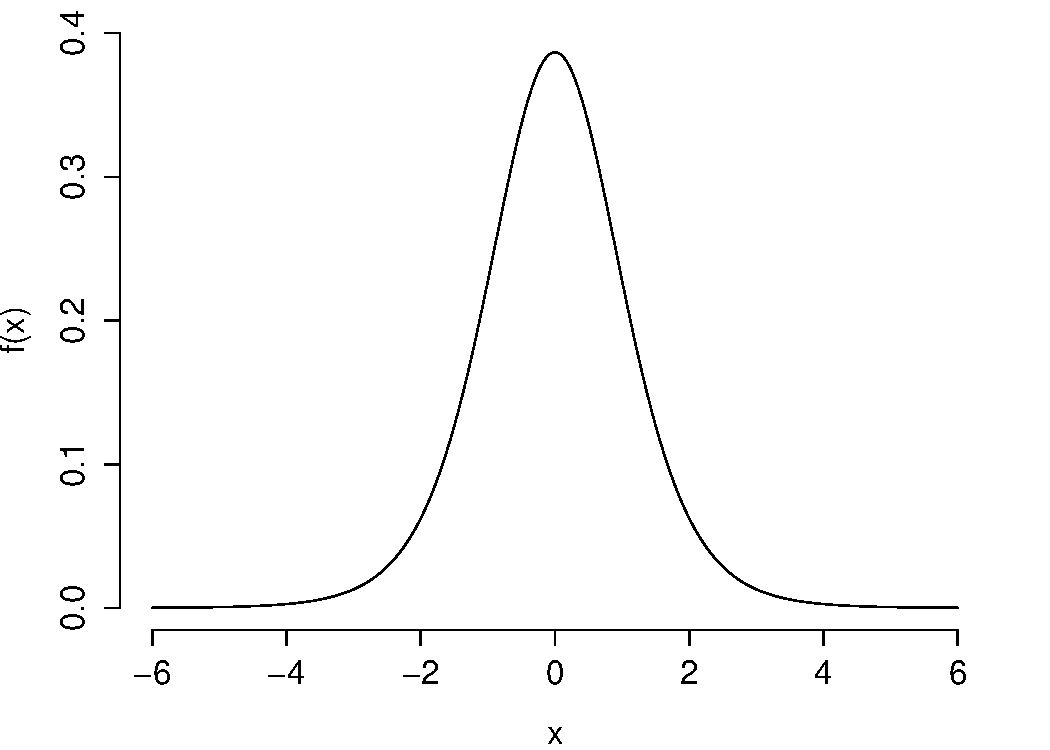
\includegraphics[scale = 0.5]{./images/t_pdf}
\end{column}

\begin{column}[r]{6cm}
$H_0\colon \mu=550 \Rightarrow \displaystyle \frac{\bar{X}_n - 550}{S/\sqrt{n}} \sim t(n-1)$\\ \pause
\vspace{1em}
One-sided Alternative $H_1\colon \mu > 550$\\ \pause
\vspace{1em}
Two-sided Alternative $H_1\colon \mu \neq 550$ 
\end{column}

\end{columns}
 
\end{frame}
%%%%%%%%%%%%%%%%%%%%%%%%%%%%%%%%%%%%%%%%


\begin{frame}
\frametitle{What Form Should the Decision Rule Take?}
Suppose we take a random sample of $n$ Big Macs and measure their caloric content. Assume that the population is normal: $X_1, \hdots, X_n \sim \mbox{iid } N(\mu, \sigma^2)$ 
\begin{block}{Common Null Hypothesis $H_0\colon \mu = 550$}
Under $H_0$, $T_n = \sqrt{n}(\bar{X}_n - 550)/S \sim t(n-1)$ 
\end{block}
\begin{block}{One-sided Alternative $H_1\colon \mu > 550$}
Reject $H_0$ if $T_n$ is ``too big'' 
\end{block}
\begin{block}{Two-sided Alternative $H_1\colon \mu \neq 550$} 
Reject $H_0$ if $T_n$ is ``too big'' or ``too small''
\end{block}
\end{frame}

%%%%%%%%%%%%%%%%%%%%%%%%%%%%%%%%%%%%%%%%
\begin{frame}
\frametitle{One-sided Alternative $H_1\colon \mu > 550$}
The critical value is chosen to reflect both the alternative hypothesis and the significance level. 
\begin{figure}
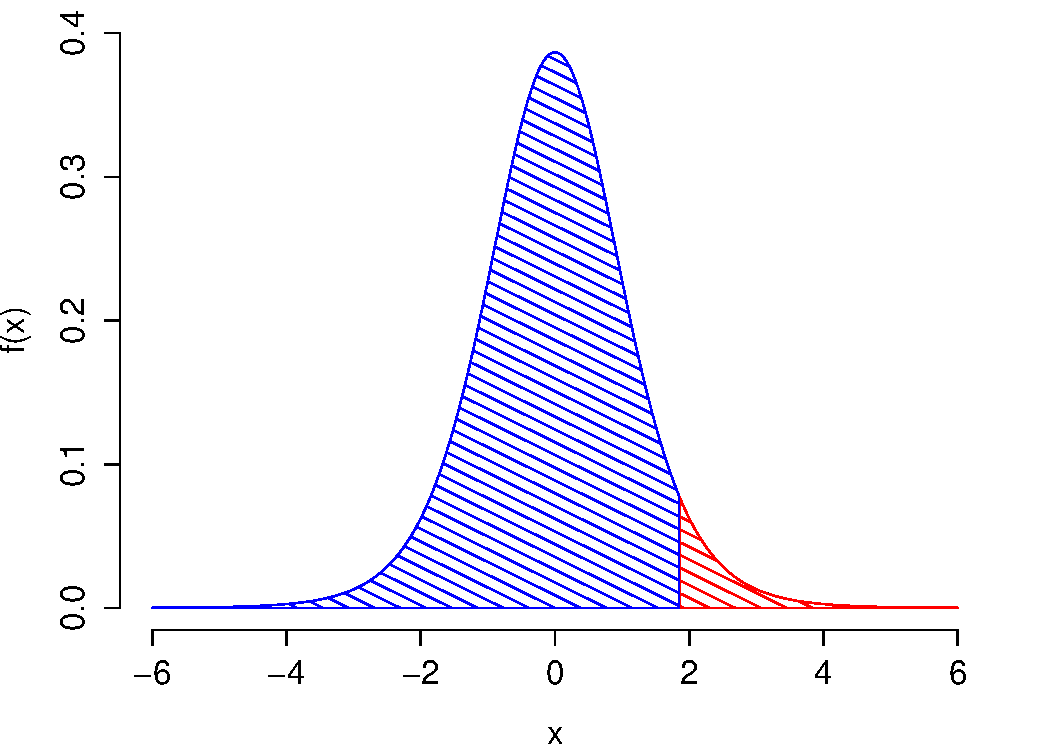
\includegraphics[scale = 0.45]{./images/one_side}
\end{figure}
One-sided Critical Value: \texttt{qt($1-\alpha$, df  = $n-1$)}
\end{frame}


%%%%%%%%%%%%%%%%%%%%%%%%%%%%%%%%%%%%%%%%

\begin{frame}
\frametitle{Two-sided Alternative $H_1\colon \mu \neq 550$}
The critical value is chosen to reflect both the alternative hypothesis and the significance level. 
\begin{figure}
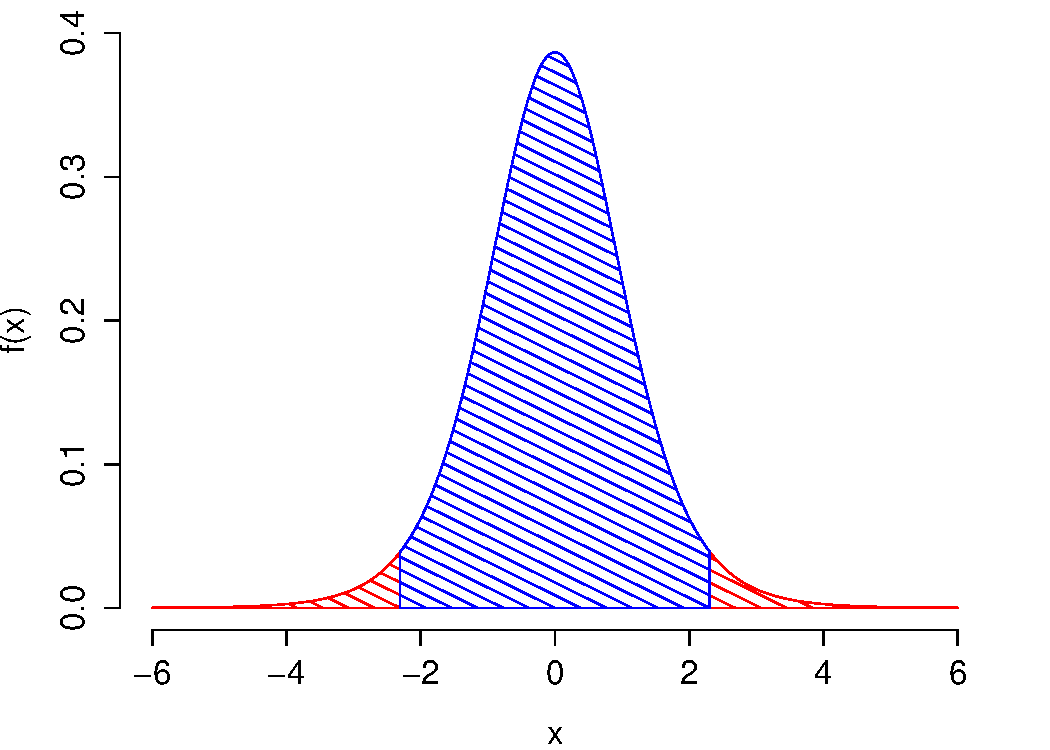
\includegraphics[scale = 0.45]{./images/two_side}
\end{figure}
Two-sided Critical Value: \texttt{qt($1-\alpha/2$, df  = $n-1$)}
\end{frame}

%%%%%%%%%%%%%%%%%%%%%%%%%%%%%%%%%%%%%%%%
\begin{frame}
Suppose, for example, $\alpha = 0.05$, $n = 9$
	\begin{eqnarray*}
		&&\texttt{qt(0.95, df  = 8)}\approx 1.86\\
		 &&\texttt{qt(0.975, df  = 8)}\approx 2.3
	\end{eqnarray*}
\begin{figure}
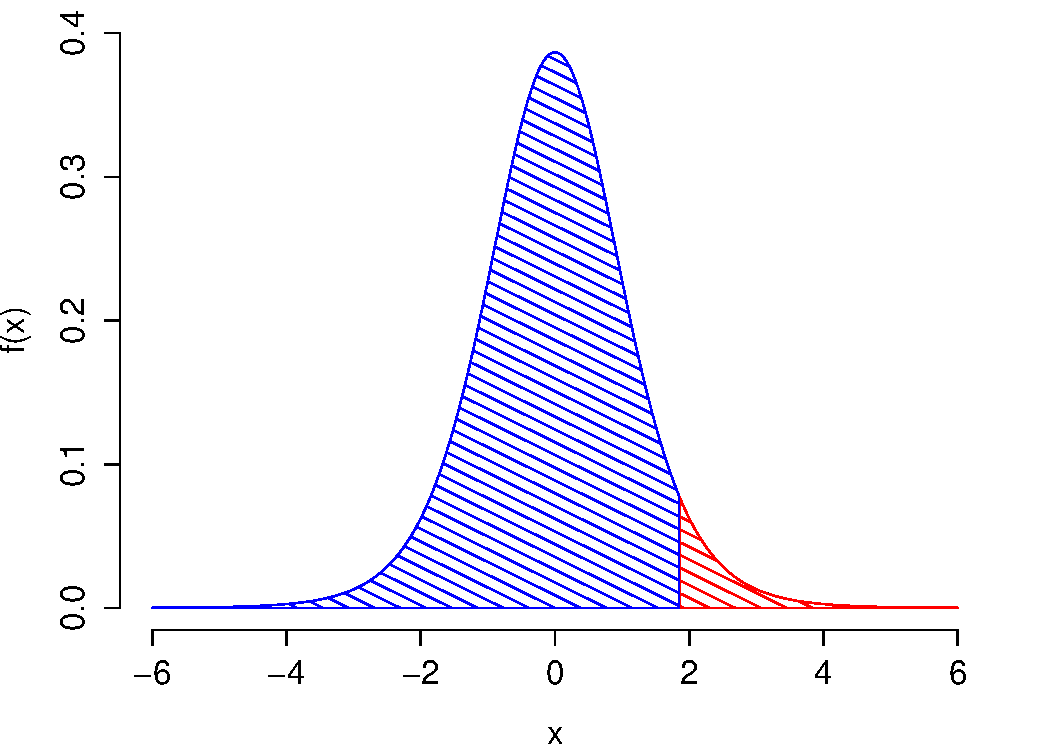
\includegraphics[scale = 0.3]{./images/one_side}
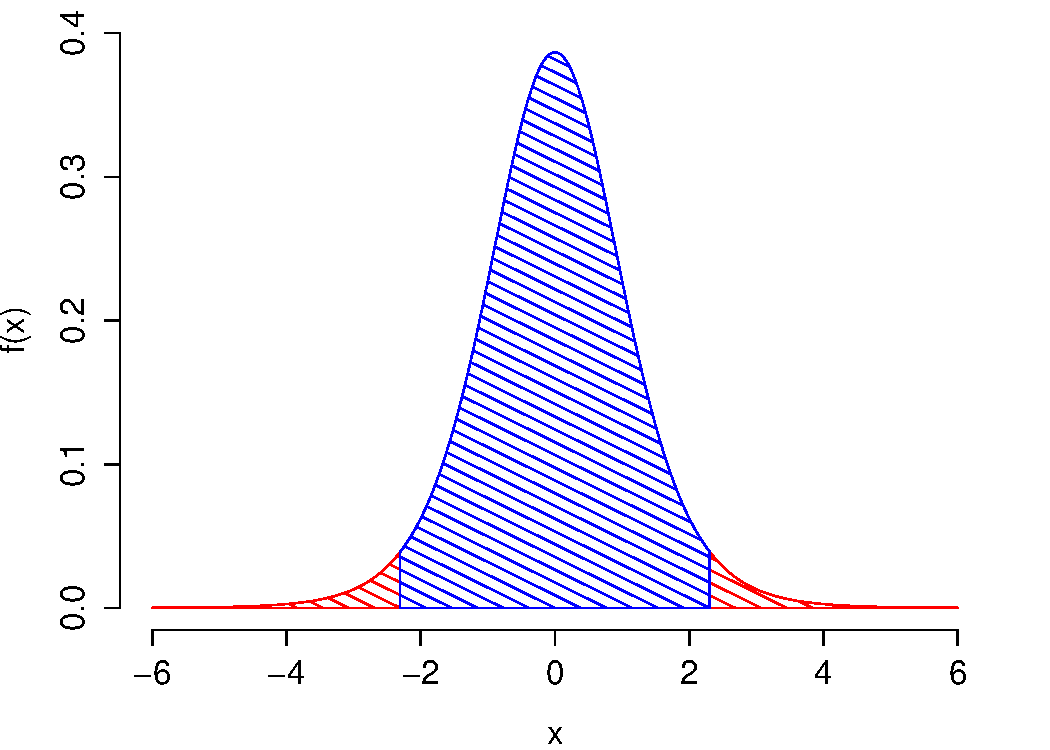
\includegraphics[scale = 0.3]{./images/two_side}
\end{figure}
One-sided Alternative: Reject $H_0$ if $\sqrt{n}(\bar{X}_n - 550)/S \geq 1.86$\\
\vspace{0.5em}
Two-sided Alternative: Reject $H_0$ if $\left|\sqrt{n}(\bar{X}_n - 550)/S\right| \geq 2.3$\\

\end{frame}

%%%%%%%%%%%%%%%%%%%%%%%%%%%%%%%%%%%%%%%%
\begin{frame}
\frametitle{Example with Simulated Data: $\alpha = 0.05$}
Suppose $n=9$, $\bar{x} = 563$, $s = 34$. What is the test statistic?


\vspace{1em}
	$$\frac{563 - 550}{34/\sqrt{9}}= \frac{13}{34/3} \approx 1.14$$



One-sided Alternative: Reject $H_0$ if $T_n\geq 1.86$\\
Two-sided Alternative: Reject $H_0$ if $\left|T_n\right| \geq 2.3$\\

\vspace{1em}
\alert{In this example, we would fail to reject $H_0$ in either case.}
\end{frame}
%%%%%%%%%%%%%%%%%%%%%%%%%%%%%%%%%%%%%%%%
\begin{frame}
\begin{center}
\huge Decision Rule and Critical Value Depend on Which Alternative We Have Specified!
\end{center}
\end{frame}

%%%%%%%%%%%%%%%%%%%%%%%%%%%%%%%%%%%%%%%%

\begin{frame}
\begin{alertblock}{Alternate Step 3}
Instead of calculating a critical value for a fixed significance level ($\alpha$), calculate the \emph{P-Value}, the minimum significance level at which we would reject the null hypothesis given the observed data.
\end{alertblock}


\end{frame}

%%%%%%%%%%%%%%%%%%%%%%%%%%%%%%%%%%%%%%%%
\begin{frame}
\frametitle{What is the p-value? (One-sided Test)}
\footnotesize
Recall: p-value is \emph{smallest significance level} at which our observed test statistic would cause us to reject $H_0$. \alert{Test statistic is $1.14$. What is the one-sided p-value? }
\begin{figure}
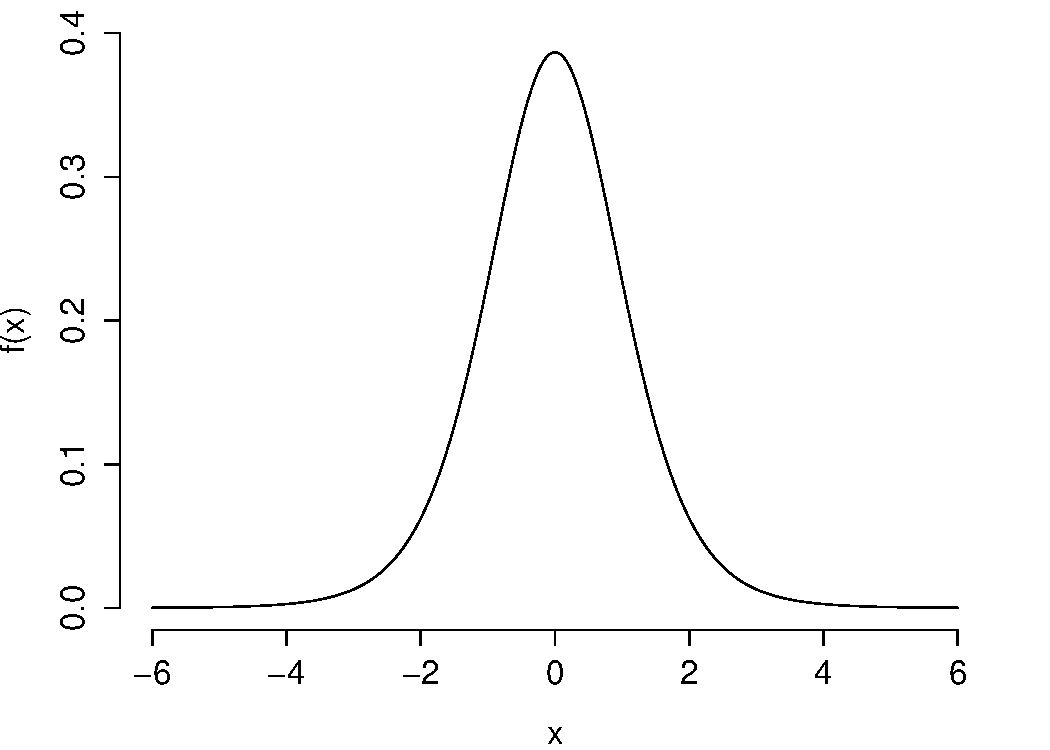
\includegraphics[scale= 0.4]{./images/p_upper1}

\end{figure}

\end{frame}

%%%%%%%%%%%%%%%%%%%%%%%%%%%%%%%%%%%%%%%%
\begin{frame}
\frametitle{What is the p-value? (One-sided Test)}
\footnotesize
Recall: p-value is \emph{smallest significance level} at which our observed test statistic would cause us to reject $H_0$. \alert{Test statistic is $1.14$. What is the one-sided p-value? }
\begin{figure}
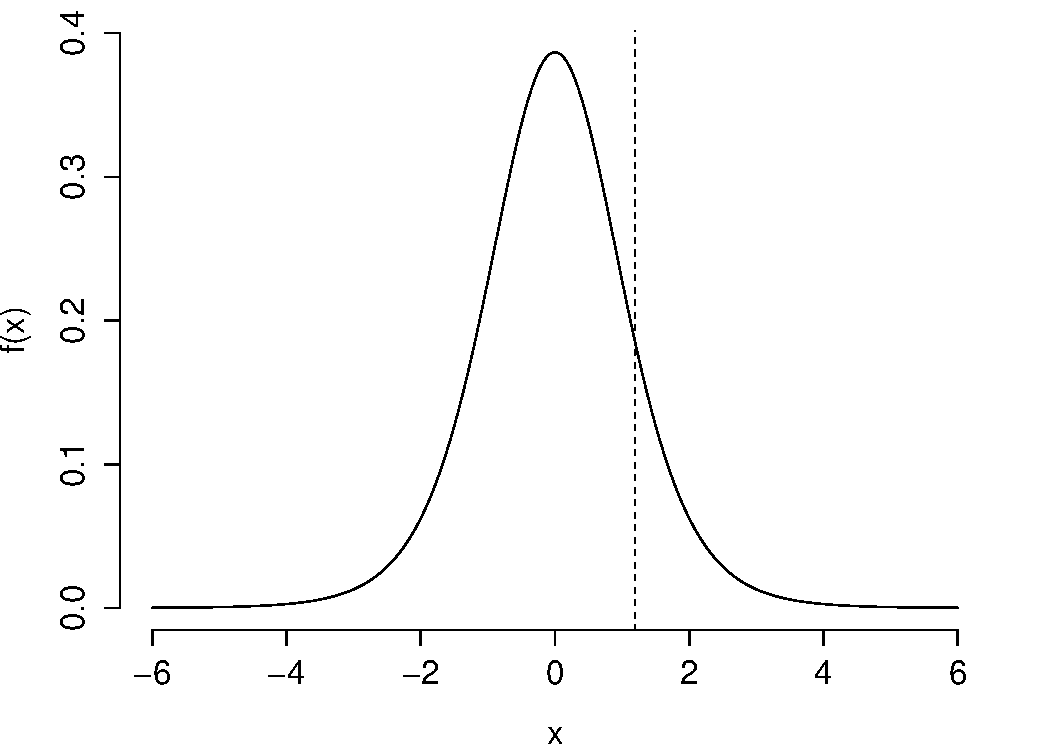
\includegraphics[scale= 0.4]{./images/p_upper2}

\end{figure}

\end{frame}

%%%%%%%%%%%%%%%%%%%%%%%%%%%%%%%%%%%%%%%%
\begin{frame}
\frametitle{What is the p-value? (One-sided Test)}
\footnotesize
Recall: p-value is \emph{smallest significance level} at which our observed test statistic would cause us to reject $H_0$. \alert{Test statistic is $1.14$. What is the one-sided p-value? }
\begin{figure}
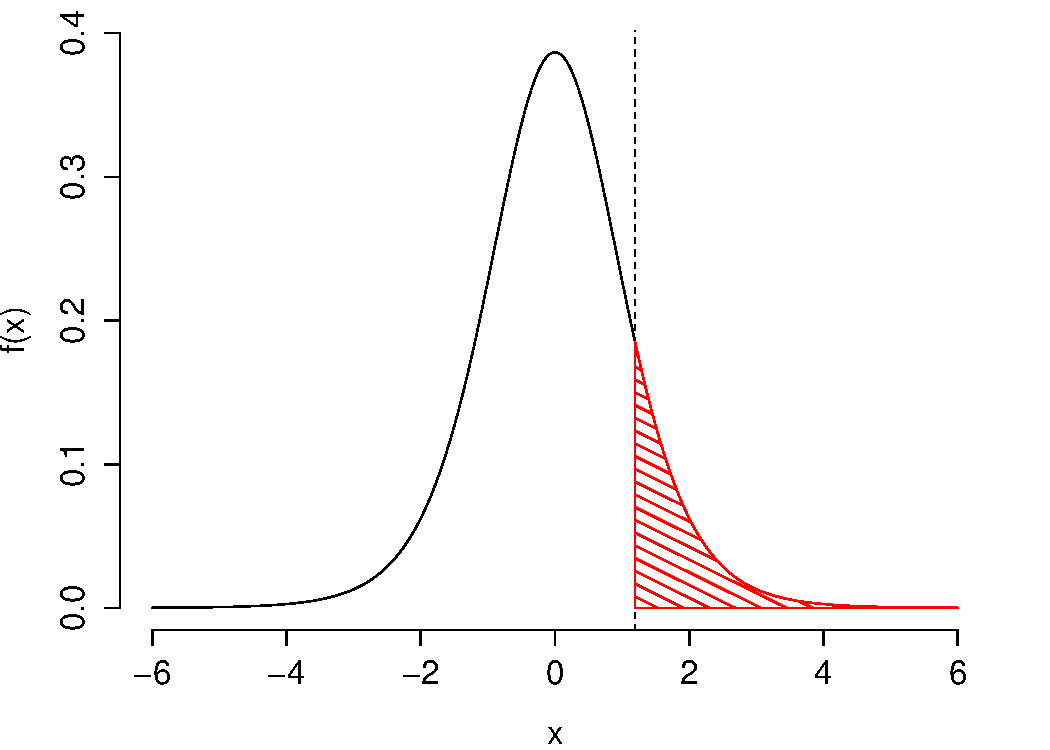
\includegraphics[scale= 0.4]{./images/p_upper3}

\end{figure}

\end{frame}

%%%%%%%%%%%%%%%%%%%%%%%%%%%%%%%%%%%%%%%%
\begin{frame}
\frametitle{What is the p-value? (One-sided Test)}
\footnotesize
Recall: p-value is \emph{smallest significance level} at which our observed test statistic would cause us to reject $H_0$. \alert{Test statistic is $1.14$. What is the one-sided p-value? }
\begin{figure}
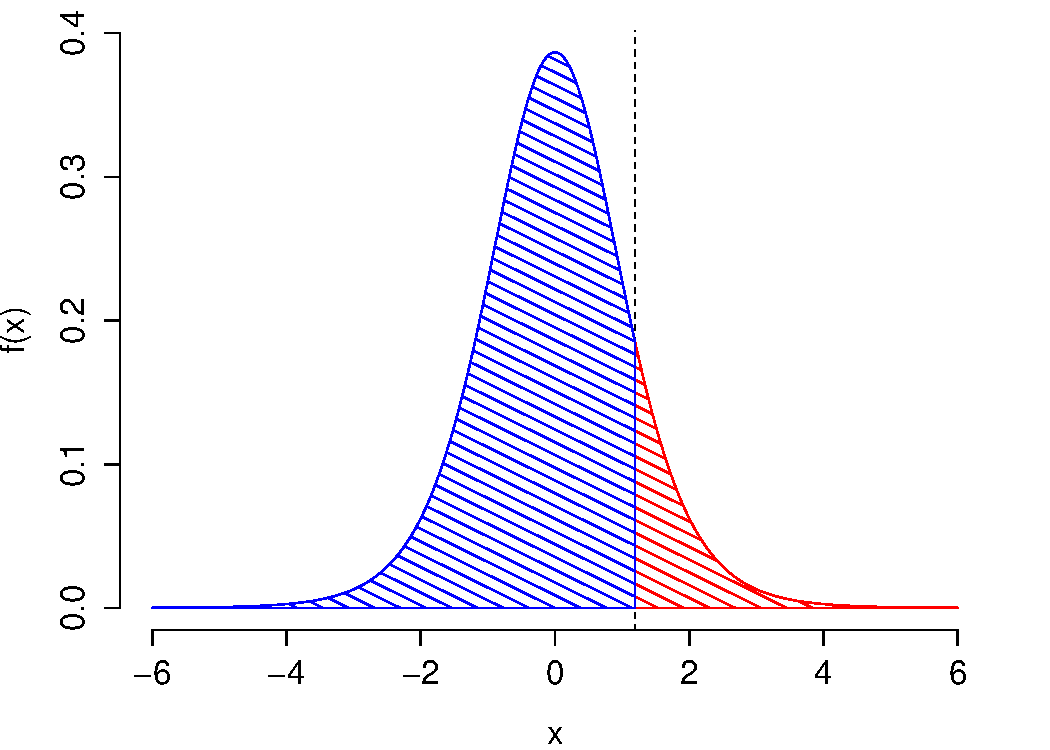
\includegraphics[scale= 0.4]{./images/p_upper4}

\end{figure}

\end{frame}

%%%%%%%%%%%%%%%%%%%%%%%%%%%%%%%%%%%%%%%%
\begin{frame}
\frametitle{What is the p-value? (One-sided Test)}
\footnotesize
Recall: p-value is \emph{smallest significance level} at which our observed test statistic would cause us to reject $H_0$. \alert{Test statistic is $1.14$. What is the one-sided p-value? }
\begin{figure}
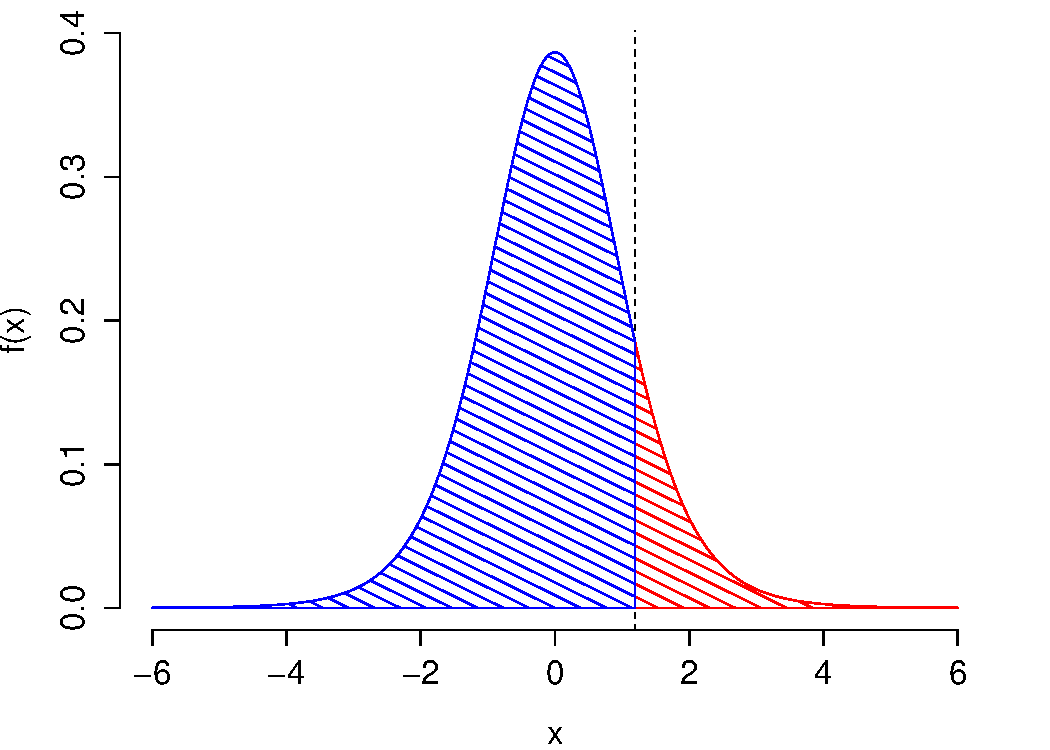
\includegraphics[scale= 0.4]{./images/p_upper4}

\end{figure}
\texttt{1 - pt(1.14, df = 8)}$\approx 0.14$
\end{frame}

%%%%%%%%%%%%%%%%%%%%%%%%%%%%%%%%%%%%%%%%
\begin{frame}
\frametitle{What is the p-value? (Two-sided Test)}
\footnotesize
Recall: p-value is \emph{smallest significance level} at which our observed test statistic would cause us to reject $H_0$. \alert{Test statistic is $1.14$. What is the two-sided p-value? }
\begin{figure}
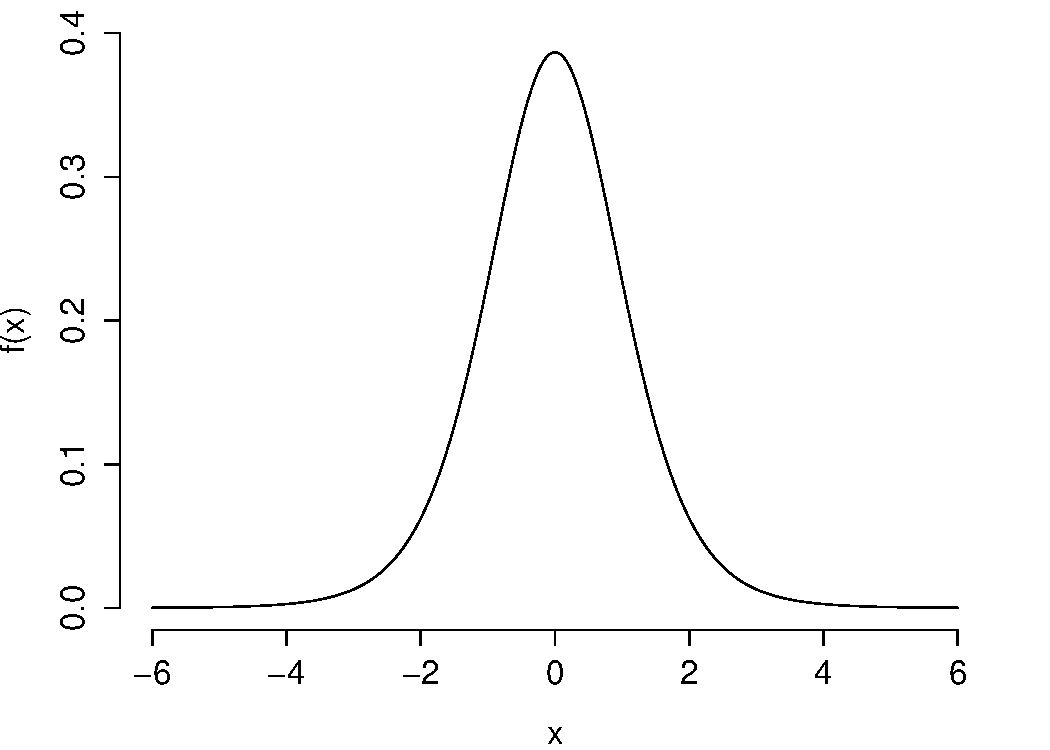
\includegraphics[scale= 0.4]{./images/p_both1}

\end{figure}

\end{frame}

%%%%%%%%%%%%%%%%%%%%%%%%%%%%%%%%%%%%%%%%
\begin{frame}
\frametitle{What is the p-value? (Two-sided Test)}
\footnotesize
Recall: p-value is \emph{smallest significance level} at which our observed test statistic would cause us to reject $H_0$. \alert{Test statistic is $1.14$. What is the two-sided p-value? }
\begin{figure}
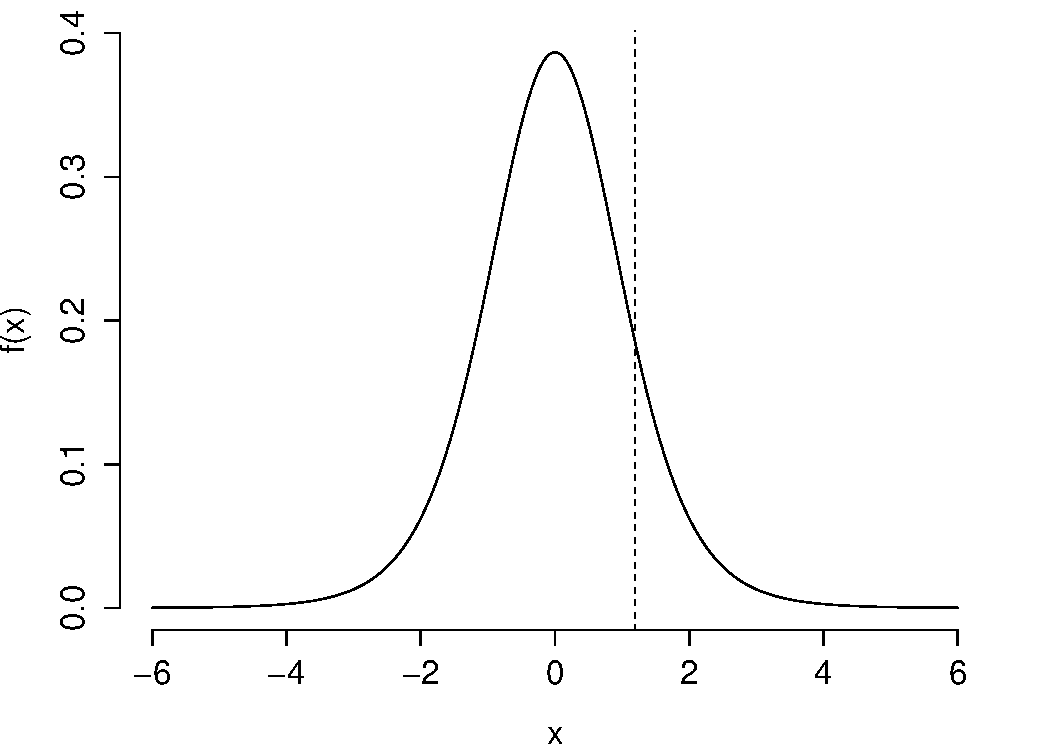
\includegraphics[scale= 0.4]{./images/p_both2}

\end{figure}

\end{frame}

%%%%%%%%%%%%%%%%%%%%%%%%%%%%%%%%%%%%%%%%
\begin{frame}
\frametitle{What is the p-value? (Two-sided Test)}
\footnotesize
Recall: p-value is \emph{smallest significance level} at which our observed test statistic would cause us to reject $H_0$. \alert{Test statistic is $1.14$. What is the two-sided p-value? }
\begin{figure}
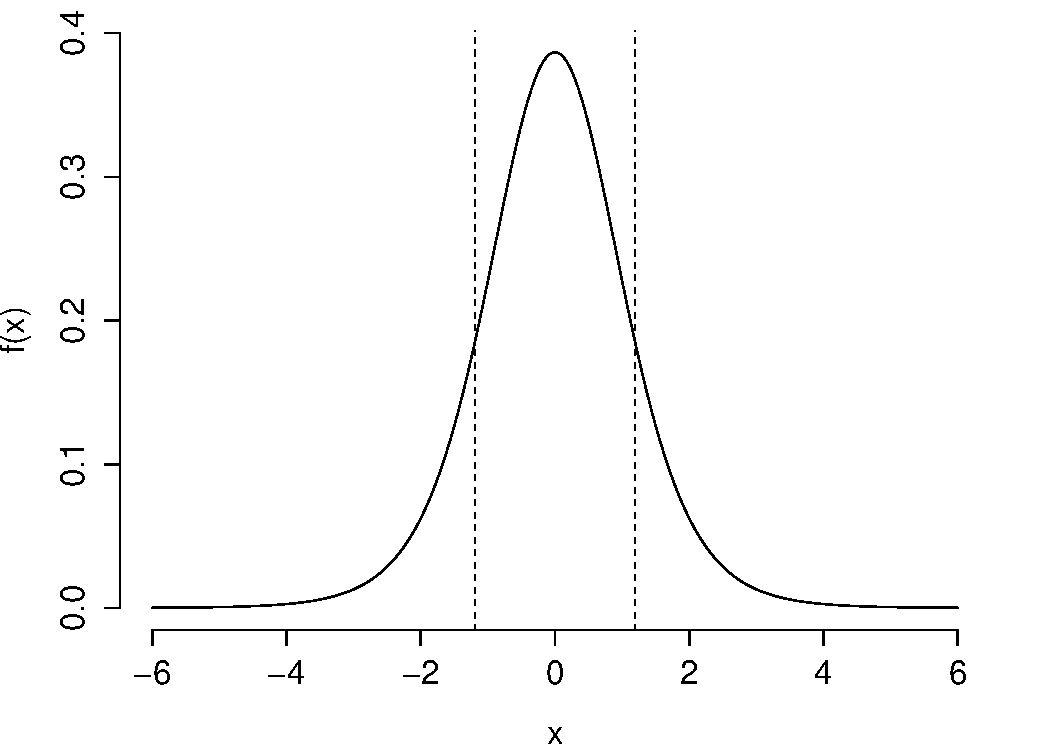
\includegraphics[scale= 0.4]{./images/p_both3}

\end{figure}

\end{frame}

%%%%%%%%%%%%%%%%%%%%%%%%%%%%%%%%%%%%%%%%
\begin{frame}
\frametitle{What is the p-value? (Two-sided Test)}
\footnotesize
Recall: p-value is \emph{smallest significance level} at which our observed test statistic would cause us to reject $H_0$. \alert{Test statistic is $1.14$. What is the two-sided p-value? }
\begin{figure}
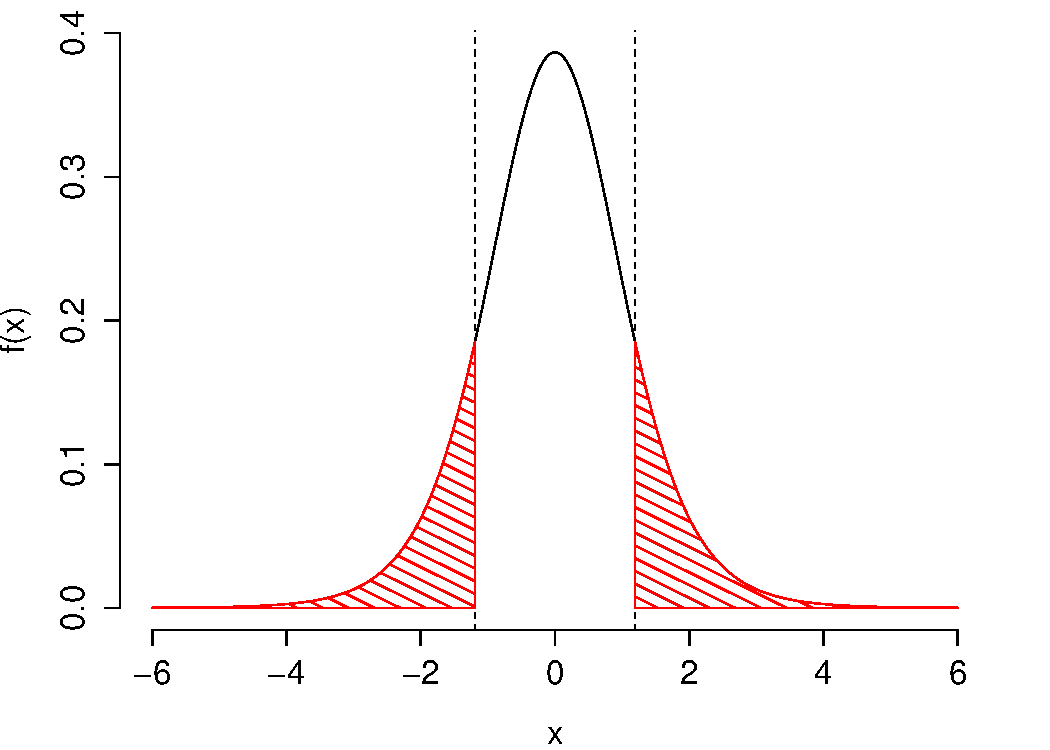
\includegraphics[scale= 0.4]{./images/p_both4}

\end{figure}

\end{frame}

%%%%%%%%%%%%%%%%%%%%%%%%%%%%%%%%%%%%%%%%
\begin{frame}
\frametitle{What is the p-value? (Two-sided Test)}
\footnotesize
Recall: p-value is \emph{smallest significance level} at which our observed test statistic would cause us to reject $H_0$. \alert{Test statistic is $1.14$. What is the two-sided p-value? }
\begin{figure}
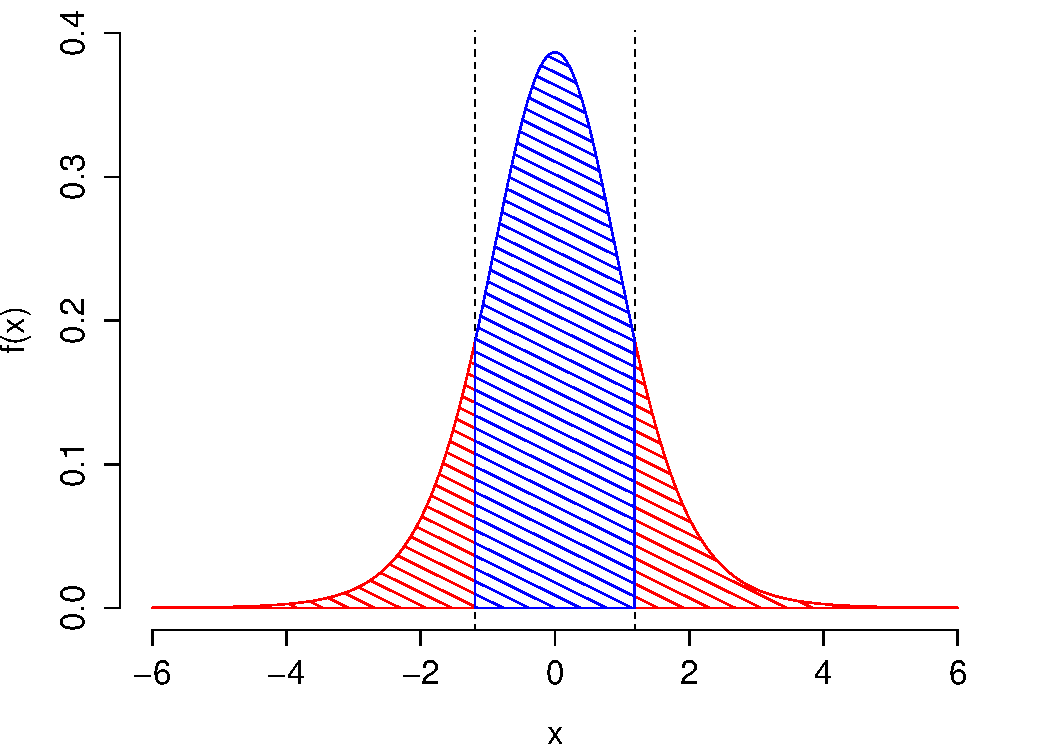
\includegraphics[scale= 0.4]{./images/p_both5}

\end{figure}

\end{frame}

%%%%%%%%%%%%%%%%%%%%%%%%%%%%%%%%%%%%%%%%
\begin{frame}
\frametitle{What is the p-value? (Two-sided Test)}
\footnotesize
Recall: p-value is \emph{smallest significance level} at which our observed test statistic would cause us to reject $H_0$. \alert{Test statistic is $1.14$. What is the two-sided p-value? }
\begin{figure}
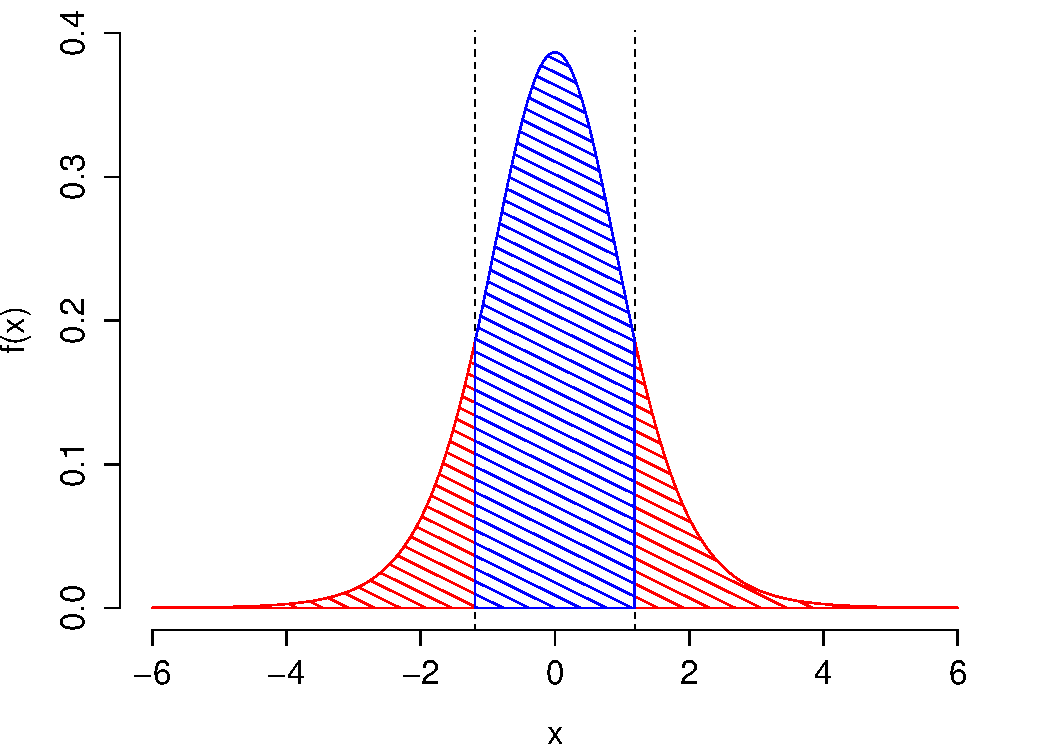
\includegraphics[scale= 0.4]{./images/p_both5}
\end{figure}

\texttt{2 * pt(-1.14, df = 8)}$\approx 0.28$ \pause \hfill \alert{This is twice the one-sided p-value!}
\end{frame}

%%%%%%%%%%%%%%%%%%%%%%%%%%%%%%%%%%%%%%%%

\begin{frame}
\frametitle{Two-sided Test is More Stringent}
\begin{block}{P-value measures strength of evidence against $H_0$}
Lower p-value means stronger evidence. 
\end{block}

\begin{block}{Two Equivalent Definitions of P-value}
	\begin{enumerate}
		\item Smallest significance level at which our observed test statistic would cause us to reject $H_0$.
		\item The probability of observing a test statistic at least as extreme as the one actually observed if $H_0$ were true.
	\end{enumerate}
\end{block}


\begin{block}{(Two-sided p-value) $= 2 \; \times$  (one-sided p-value)}
Reject $H_0$ based on two-sided test $\implies$ Reject $H_0$ based on appropriate one-sided test. The converse is \emph{false}.
\end{block}


\end{frame}
%%%%%%%%%%%%%%%%%%%%%%%%%%%%%%%%%%%%%%%%

\begin{frame}
\begin{center}
\huge P-Value Depends on Which Alternative We Have Specified!
\end{center}
\end{frame}

%%%%%%%%%%%%%%%%%%%%%%%%%%%%%%%%%%%%%%%%
\begin{frame}
\frametitle{Steps in Hypothesis Testing}

\begin{enumerate}
\item Specify Null and Alternative Hypotheses
\item Identify a Test Statistic: a function of the data and the unknown parameter that has a known sampling distribution under the null.
\item Specify a Decision Rule and a Critical Value so the Type I Error Rate equals $\alpha$.
\end{enumerate}

\begin{alertblock}{Alternative to Step 3}
	Calculate P-Value: the minimum significance level  ($\alpha$) at which we would reject $H_0$ given the observed data.
\end{alertblock}

\end{frame}


%%%%%%%%%%%%%%%%%%%%%%%%%%%%%%%%%%%%%%%%
\begin{frame}
\frametitle{How to Handle Other Examples?}

\alert{You already know lots of sampling distributions! Testing is very similar to constructing confidence intervals in that the steps are always the same, and the only thing that differs is \emph{which} sampling distribution we work with.}

\end{frame}

%%%%%%%%%%%%%%%%%%%%%%%%%%%%%%%%%%%%%%%%

%%%%%%%%%%%%%%%%%%%%%%%%%%%%%%%%%%%%%%%%


\begin{frame}
\frametitle{The Anchoring Experiment}
On the first day of class, you were each shown a random number. You were then asked what proportion of UN member states are located in Africa. 

	\begin{block}{``Hi'' Group -- Shown 65 ($n=46$)}
		Sample Mean: $30.7$, Sample Variance: $253$
\end{block}


	\begin{block}{``Lo'' Group -- Shown 10 ($m=43$)}
	Sample Mean: $17.1$, Sample Variance: $86$
\end{block}

\begin{alertblock}{What are we going to test?}
	$H_0\colon \mu_{Lo} = \mu_{Hi}$
\end{alertblock}
\end{frame}
%%%%%%%%%%%%%%%%%%%%%%%%%%%%%%%%%%%%%%%%

\begin{frame}
\frametitle{The Anchoring Experiment}
\begin{figure}
\centering
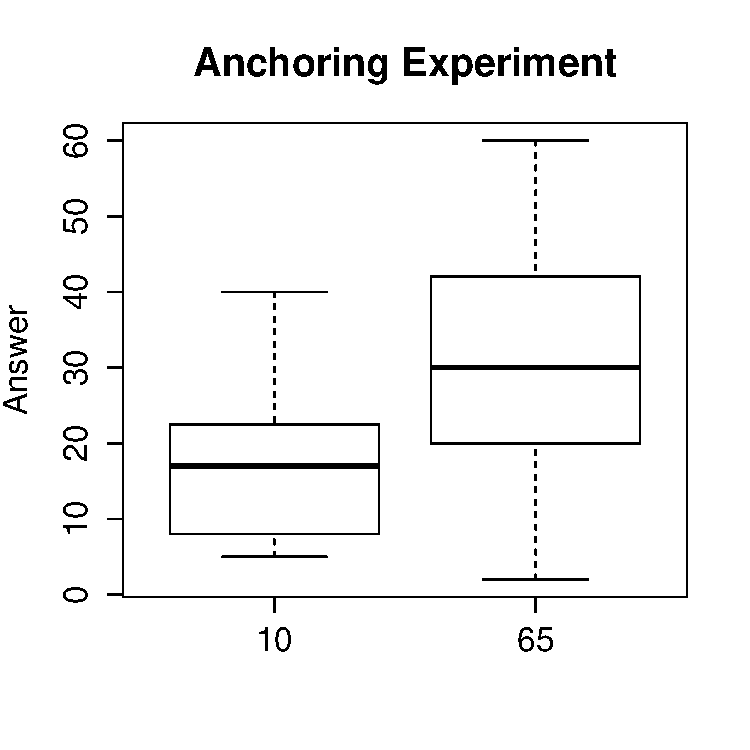
\includegraphics[scale = 0.55]{./images/anchoring_boxplot}
\end{figure}
\end{frame}
%%%%%%%%%%%%%%%%%%%%%%%%%%%%%%%%%%%%%%%%
\begin{frame}
\frametitle{What is our Test Statistic?}
\begin{block}{Sampling Distribution}
		$$\frac{\left(\bar{X}_{Hi} - \bar{X}_{Lo}\right) - \left(\mu_{Hi} - \mu_{Lo}\right)}{\sqrt{\frac{S_{Hi}^2}{n_{Hi}} + \frac{S_{Lo}^2}{n_{Lo}}}} \approx N(0,1)$$
\end{block}

\begin{block}{Test Statistic: Impose the Null}
Under $H_0\colon \mu_{Lo} = \mu_{Hi}$
	$$T_n =\frac{\bar{X}_{Hi} - \bar{X}_{Lo}}{\sqrt{\frac{S_{Hi}^2}{n_{Hi}} + \frac{S_{Lo}^2}{n_{Lo}}}} \approx N(0,1)$$
\end{block}
\end{frame}


%%%%%%%%%%%%%%%%%%%%%%%%%%%%%%%%%%%%%%%%
\begin{frame}
\frametitle{What is our Test Statistic?}
\footnotesize
$\bar{X}_{Hi} = 30.7$, $s^2_{Hi} = 253$, $n_{Hi} = 46$\\
$\bar{X}_{Lo} = 17.1$, $s^2_{Lo} = 86$, $n_{Lo} = 43$\\
\normalsize
\vspace{2em}

\begin{block}{Under $H_0\colon \mu_{Lo} = \mu_{Hi}$}
	$$T_n = \frac{\bar{X}_{Hi} - \bar{X}_{Lo}}{\sqrt{\frac{S_{Hi}^2}{n_{Hi}} + \frac{S_{Lo}^2}{n_{Lo}}}} \approx N(0,1)$$
\end{block}

\begin{block}{Plugging in Our Data}
$$T_n = \frac{\bar{X}_{Hi} - \bar{X}_{Lo}}{\sqrt{\frac{S_{Hi}^2}{n_{Hi}} + \frac{S_{Lo}^2}{n_{Lo}}}} \approx 5$$
\end{block}
\end{frame}


%%%%%%%%%%%%%%%%%%%%%%%%%%%%%%%%%%%%%%%%
\begin{frame}
\frametitle{\hfill 
\includegraphics[scale = 0.05]{./images/clicker}}
Approximately what critical value should we use to test $H_0\colon \mu_{Lo} = \mu_{Hi}$ against the two-sided alternative for this problem?


\vspace{1em}
\begin{center}
\begin{tabular}{l|lll}
$\alpha$ &   0.10& 0.05 &0.01\\
\hline
\texttt{qnorm($1-\alpha$)} & 1.28 &1.64 &2.33\\
\texttt{qnorm($1-\alpha/2$)} &1.64 &1.96& 2.58
\end{tabular}
\end{center}
\vspace{8em}
\end{frame}
%%%%%%%%%%%%%%%%%%%%%%%%%%%%%%%%%%%%%%%%
\begin{frame}
\frametitle{\hfill 
\includegraphics[scale = 0.05]{./images/clicker}}
Which of these commands would give us the p-value of our test of $H_0\colon \mu_{Lo} = \mu$ against $H_1\colon \mu_{Lo}<\mu_{Hi}$ at significance level $\alpha$?
\vspace{1em}
	\begin{enumerate}[(a)]
		\item \texttt{qnorm($1-\alpha$)}
		\item \texttt{qnorm($1-\alpha/2$)}
		\item \texttt{1 - pnorm(5)}
		\item \texttt{2 * (1 - pnorm(5))}
	\end{enumerate}
	

\end{frame}
%%%%%%%%%%%%%%%%%%%%%%%%%%%%%%%%%%%%%%%%

\begin{frame}
\frametitle{P-values for $H_0\colon \mu_{Lo} = \mu_{Hi}$}
We plug in the value of the test statistic that we observed: 5
\begin{block}{Against $H_1\colon \mu_{Lo}< \mu_{Hi}$}
\texttt{1 - pnorm(5)} $< 0.0000$
\end{block}

\begin{block}{Against $H_1\colon \mu_{Lo}\neq \mu_{Hi}$}
\texttt{2 * (1 - pnorm(5))} $< 0.0000$
\end{block}

\vspace{1em}

\alert{If the null is true (the two population means are equal) it would be extremely unlikely to observe a test statistic as large as this!}

\end{frame}


%%%%%%%%%%%%%%%%%%%%%%%%%%%%%%%%%%%%%%%%

\begin{frame}
\frametitle{Hypothesis Testing Part III}
	\begin{enumerate}
\item Example: Which Exam was Harder?
\item Relationship Between Testing and CIs
\item Tests for Proportions 
\item \alert{Statistical Power}
\end{enumerate}
\end{frame}

%%%%%%%%%%%%%%%%%%%%%%%%%%%%%%%%%%%%%%%%
\begin{frame}
\frametitle{Which Exam is Harder?}
% latex.default(round(grades.out, 1), file = "grades.tex", rowname = NULL) 
%
\begin{table}[!tbp]
\begin{center}
\begin{tabular}{rccr}
\hline\hline
\multicolumn{1}{r}{Student}&\multicolumn{1}{c}{Exam 1}&\multicolumn{1}{c}{Exam 2}&\multicolumn{1}{r}{Difference}\tabularnewline
\hline
$ 1$&$57.1$&$60.7$&$  3.6$\tabularnewline
\vdots&\vdots&\vdots&\vdots\\
$71$&$78.6$&$82.9$&$  4.3$\tabularnewline
\hline
Sample Mean: & 79.6 & 81.4  &1.8\\
Sample Var. &117  & 151 & 124\\
Sample Corr.& \multicolumn{2}{c}{0.54}&\\
\hline
\end{tabular}
\end{center}
\end{table}

\end{frame}
%%%%%%%%%%%%%%%%%%%%%%%%%%%%%%%%%%%%%%%%
\begin{frame}
\frametitle{One-Sample Hypothesis Test Using Differences}
\small
\fbox{Let $D_i = X_i - Y_i$ be (Midterm 2 Score - Midterm 1 Score) for student $i$}
\vspace{0.1em}
\begin{block}{Null Hypothesis}
$H_0\colon \mu_1 = \mu_2$, i.e.\ both exams were of the same difficulty
\end{block}
\begin{block}{Two-Sided Alternative}
$H_1\colon \mu_1 \neq \mu_2$, i.e.\ one exam was harder than the other
\end{block}
\begin{block}{One-Sided Alternative}
$H_1\colon \mu_2 > \mu_1$, i.e.\ the second exam was easier
\end{block}
% \begin{block}{Test Statistic}
% Under $H_0$ this has an approx.\ standard normal distribution by the CLT:
% 	$$\displaystyle \frac{\bar{D}_n}{\widehat{SE}(\bar{D}_n)}=  \frac{1.8}{\sqrt{124/71}}  \approx \alert{1.36} $$
% \end{block}
%\alert{Approximate 95\% CI Based on the CLT:}
%$$\alert{\boxed{1.8 \pm 2.6 = (-0.8, 4.4)}} \quad \mbox{What is our conclusion?}$$

\end{frame}
%%%%%%%%%%%%%%%%%%%%%%%%%%%%%%%%%%%%%%%%

\begin{frame}
\frametitle{Decision Rules}
\small
\fbox{Let $D_i = X_i - Y_i$ be (Midterm 2 Score - Midterm 1 Score) for student $i$}
\vspace{0.1em}


\begin{block}
	{Test Statistic}
$$\displaystyle \frac{\bar{D}_n}{\widehat{SE}(\bar{D}_n)}=\frac{1.8}{\sqrt{124/71}} \approx 1.36$$
\end{block}


\begin{block}{Two-Sided Alternative} 
Reject $H_0\colon \mu_1 = \mu_2$ in favor of $H_1\colon \mu_1 \neq \mu_2$ if $|\bar{D}_n|$ is sufficiently large.
\end{block}
\begin{block}{One-Sided Alternative}
Reject $H_0\colon \mu_1 = \mu_2$ in favor of $H_1\colon \mu_2 >\mu_1$ if $\bar{D}_n$ is sufficiently large.
\end{block}
\end{frame}
%%%%%%%%%%%%%%%%%%%%%%%%%%%%%%%%%%%%%%%%

\begin{frame}
\frametitle{Reject against \emph{Two-sided} Alternative with $\alpha = 0.1$?  
\includegraphics[scale = 0.05]{./images/clicker}}

	$$\boxed{\displaystyle \frac{\bar{D}_n}{\widehat{SE}(\bar{D}_n)}= \frac{1.8}{\sqrt{124/71}} \approx 1.36} $$

\begin{center}
\begin{tabular}{l|lll}
$\alpha$ &   0.10& 0.05 &0.01\\
\hline
\texttt{qnorm($1-\alpha$)} & 1.28 &1.64 &2.33\\
\texttt{qnorm($1-\alpha/2$)} &1.64 &1.96& 2.58
\end{tabular}
\end{center}

\begin{enumerate}[(a)]
\item Reject
\item Fail to Reject
\item Not Sure
\end{enumerate}

\end{frame}

%%%%%%%%%%%%%%%%%%%%%%%%%%%%%%%%%%%%%%%%
\begin{frame}
\frametitle{Reject against \emph{One-sided} Alternative with $\alpha = 0.1$?  
\includegraphics[scale = 0.05]{./images/clicker}}

	$$\boxed{\displaystyle \frac{\bar{D}_n}{\widehat{SE}(\bar{D}_n)}= \frac{1.8}{\sqrt{124/71}} \approx 1.36} $$

\begin{center}
\begin{tabular}{l|lll}
$\alpha$ &   0.10& 0.05 &0.01\\
\hline
\texttt{qnorm($1-\alpha$)} & 1.28 &1.64 &2.33\\
\texttt{qnorm($1-\alpha/2$)} &1.64 &1.96& 2.58
\end{tabular}
\end{center}

\begin{enumerate}[(a)]
\item Reject
\item Fail to Reject
\item Not Sure
\end{enumerate}



\end{frame}

%%%%%%%%%%%%%%%%%%%%%%%%%%%%%%%%%%%%%%%%
\begin{frame}
\frametitle{P-Values for the Test of $H_0\colon \mu_1 = \mu_2$}

	$$\boxed{\displaystyle \frac{\bar{D}_n}{\widehat{SE}(\bar{D}_n)}= \frac{1.8}{\sqrt{124/71}} \approx 1.36} $$

\begin{block}{One-Sided $H_1\colon \mu_2 > \mu_1 $} 
$\texttt{1 - pnorm(1.36)} =  \texttt{pnorm(-1.36)}  \approx 0.09$ 
\end{block}

\begin{block}{Two-Sided $H_1 \colon \mu_1 \neq \mu_2$} 
$\texttt{2 * (1 - pnorm(1.36))} =  \texttt{2 * pnorm(-1.36)} \approx 0.18$
\end{block}
\end{frame}
%%%%%%%%%%%%%%%%%%%%%%%%%%%%%%%%%%%%%%%%


\begin{frame}
\frametitle{Relationship between CI and Two-sided Test}
Suppose $X_1, \hdots, X_n \sim \mbox{iid } N(\mu,\sigma^2)$

\vspace{1em}
	\begin{block}{Test $H_0\colon \mu = \mu_0$ vs.\ $H_1\colon \mu \neq \mu_0$ at significance level $\alpha$} 
		\begin{itemize}
			\item Test Statistic:  $T_n = \sqrt{n}(\bar{X}_n - \mu_0)/S \sim t(n-1)$ under $H_0$ 
			\item Decision Rule: Reject $H_0$ if $|T_n| > \texttt{qt}(1-\alpha/2, \texttt{df}=n-1)$ 
			\end{itemize}

			\pause
\end{block}
	\begin{block}{$100\times (1-\alpha)\%$ CI for $\mu$} 
		$$\bar{X}_n \pm \texttt{qt}(1-\alpha/2, \texttt{df}=n-1) \frac{S}{\sqrt{n}}$$
\end{block}
\end{frame}
%%%%%%%%%%%%%%%%%%%%%%%%%%%%%%%%%%%%%%%%
\begin{frame}
\frametitle{Relationship between CI and Two-sided Test}
$\alert{c =  \texttt{qt}(1-\alpha/2, \texttt{df}=n-1)}$
\begin{block}{Decision Rule: Reject $H_0$ if}
		$$\left|\frac{\bar{X}_n - \mu_0}{S/\sqrt{n}} \right|> c \quad \iff \pause  \quad \left(\frac{\bar{X}_n - \mu_0}{S/\sqrt{n}}> c \;\;\mbox{  \alert{OR}  }\;\;\frac{\bar{X}_n - \mu_0}{S/\sqrt{n}}< - c\right)$$
\end{block}

\pause
\begin{block}{Equivalent to: \emph{Don't Reject} $H_0$ provided}
	$$-c \leq \frac{\bar{X}_n - \mu_0}{S/\sqrt{n}}\leq c $$ \pause
	$$\alert{\bar{X_n} - c\times \frac{S}{\sqrt{n}} \leq \mu_0 \leq \bar{X_n} + c\times \frac{S}{\sqrt{n}}}$$
\end{block}
\end{frame}
%%%%%%%%%%%%%%%%%%%%%%%%%%%%%%%%%%%%%%%%
\begin{frame}
\frametitle{What does this mean?}

\begin{block}
	{Two-sided Test $\iff$ Checking if $\mu_0 \in$ CI}
	A two-sided test of $H_0\colon \mu = \mu_0$ against $H_1\colon \mu\neq \mu_0 $ at significance level $\alpha$ is equivalent to checking whether $\mu_0$ lies inside the corresponding $100\times (1-\alpha)\%$ confidence interval for $\mu$.
\end{block}

\pause

\begin{block}
	{``Inverting'' Two-sided Test to get a CI}	
	Collect all the values $\mu_0$ such that we cannot reject $H_0\colon \mu = \mu_0$ against the two-sided alternative. The result is \emph{precisely} a $100\times (1-\alpha)\%$ CI for $\mu$.
\end{block}
\end{frame}
%%%%%%%%%%%%%%%%%%%%%%%%%%%%%%%%%%%%%%%%

\begin{frame}
\frametitle{Tests and CIs for Proportions}
\footnotesize
Suppose $X_1, \hdots, X_n \sim \mbox{iid Bernoulli}(p)$ indep.\ of $Y_1, \hdots, Y_m \sim \mbox{iid Bernoulli}(q)$.\\
\normalsize
\vspace{1em}

From the CLT:
	$$\frac{\hat{p} - p}{\sqrt{\frac{\hat{p}(1-\hat{p})}{n}}} \approx N(0,1)$$
and
$$\frac{(\hat{p} - \hat{q}) - (p-q)}{\sqrt{\frac{\hat{p}(1-\hat{p})}{n} + \frac{\hat{q}(1-\hat{q})}{m}}} \approx N(0,1)$$

\alert{We can use these results for both testing and building CIs}
\end{frame}
%%%%%%%%%%%%%%%%%%%%%%%%%%%%%%%%%%%%%%%%
\begin{frame}
\frametitle{``Textbook'' CIs for Proportions}
	$$\widehat{p} \pm \texttt{qnorm}(1 - \alpha/2) \times \sqrt{\frac{\hat{p}(1-\hat{p})}{n}}$$
	
	$$\left(\widehat{p} -\widehat{q}\right)\pm \texttt{qnorm}(1 - \alpha/2) \times \sqrt{\frac{\hat{p}(1-\hat{p})}{n} + \frac{\hat{q}(1-\hat{q})}{m}}$$
\end{frame}
%%%%%%%%%%%%%%%%%%%%%%%%%%%%%%%%%%%%%%%%
\begin{frame}
	\frametitle{``Unrefined'' Tests for Proportions -- Like Tests for Means}
	$$H_0\colon p = p_0 \Rightarrow \frac{\hat{p} - p_0}{\sqrt{\frac{\hat{p}(1-\hat{p})}{n}}} \approx N(0,1)$$
	\vspace{1em}
	
	$$H_0\colon p = q \Rightarrow \frac{\hat{p} - \hat{q}}{\sqrt{\frac{\hat{p}(1-\hat{p})}{n} + \frac{\hat{q}(1-\hat{q})}{m}}} \approx N(0,1)$$
\end{frame}
%%%%%%%%%%%%%%%%%%%%%%%%%%%%%%%%%%%%%%%%
\begin{frame}
\frametitle{Refined Tests for Proportions: Fully Impose $H_0$}

\begin{block}{Under $H_0$ we know something about the standard error!}
For proportions, mean and SE are are linked!
\end{block}
\begin{block}{One-sample: SE Known under $H_0$}
	$$H_0\colon p = p_0 \Rightarrow \frac{\hat{p} - p_0}{\sqrt{\frac{p_0(1-p_0)}{n}}} \approx N(0,1)$$
\end{block}
	\pause
\begin{block}{Two-sample: Pooled SE estimator under $H_0$}
	$$H_0\colon p = q \Rightarrow \frac{\hat{p} - \hat{q}}{\sqrt{\left(\frac{1}{n} + \frac{1}{m} \right)\widehat{\pi}(1-\widehat{\pi})}} \approx N(0,1)$$
	where $\widehat{\pi} = \frac{n\widehat{p} + m\widehat{q}}{n+m}$
\end{block}
\end{frame}
%%%%%%%%%%%%%%%%%%%%%%%%%%%%%%%%%%%%%%%%
% \begin{frame}
% \frametitle{Refined Test and Refined CI}
% \small
% \begin{block}{Refined Test Imposes $H_0$ in \emph{both} Numerator \& Denominator}
% Our procedures for proportions are approximations based on the CLT. (The population in question is actually Bernoulli!) Fully imposing the null, as on the previous slide, makes the approximation work better.
% \end{block}

% \pause

% \begin{block}{Ideally Invert Refined Test to get CI}
% Earlier in this lecture, we talked about how the set of all parameter values that are not rejected by a two-sided test with significance level $\alpha$ gives a $100\times(1-\alpha)\%$ CI. Ideally, we could invert the refined tests for proportions to get \emph{corresponding} refined CIs. The math required for this, however, is a little tricky.
% \end{block}

% \end{frame}
% %%%%%%%%%%%%%%%%%%%%%%%%%%%%%%%%%%%%%%%%
\begin{frame}
	\frametitle{``Refined'' Procedures for Proportions}
\begin{columns}
	\column{0.45\textwidth}
	\begin{block}
		{Refined CI}
		Add four ``fake'' observations.
	\end{block}
	\column{0.45\textwidth}
		\begin{block}
			{Refined Test} Fully impose $H_0$ in $T_n$
		\end{block}
\end{columns}

\vspace{2em}

\begin{block}
	{What's Going on Here?}
		\begin{itemize}
		\item $X_1, \hdots, X_n \sim \mbox{ iid Bernoulli}(p)$ has special structure:
			\begin{enumerate}
				\item Discrete Data (zeros and ones)
				\item Single Population parameter $p$ 
			\end{enumerate}
		\item Use this structure to improve the approximation of the CLT
		\item Turns out that the refined CI is approximately what you get from inverting the corresponding refined test.
	\end{itemize}
\end{block}
\end{frame}

%%%%%%%%%%%%%%%%%%%%%%%%%%%%%%%%%%%%%%%%
% \begin{frame}
% \frametitle{Refined Test and Refined CI}
% \small
% \begin{block}{Inverting \emph{Unrefined Tests} Gives Textbook CI}
% The \emph{unrefined} tests for proportions do not use the fact that, under the null, we actually have some additional information regarding the standard errors. If we invert these tests, we get the textbook confidence intervals studied earlier (see preceding slides). 
% \end{block}

% \pause

% \begin{block}{Refined CIs are an \emph{Approximation} to Inverting Refined Tests}
% A few lectures ago, we talked about the refined CIs for proportions that involved adding ``fake'' observations to the data. These are \emph{very close} to what you get if you inverted the refined tests. \alert{This is why we use them.}
% \end{block}

% \pause

% \vspace{1em} 
% \large
% \alert{Unless instructed otherwise, you should \emph{always} use the refined tests and refined CIs when working with proportions: they work better.}

% \end{frame}
% %%%%%%%%%%%%%%%%%%%%%%%%%%%%%%%%%%%%%%%%
\begin{frame}
\frametitle{What is a Type I Error? 
\includegraphics[scale = 0.05]{./images/clicker}}

\begin{enumerate}[(a)]
	\item Rejecting a false Null
	\item Failing to Reject a True Null
	\item Rejecting a True Null
	\item Failing to Reject a False Null
\end{enumerate}

\end{frame}


%%%%%%%%%%%%%%%%%%%%%%%%%%%%%%%%%%%%%%%%
\begin{frame}
\frametitle{What is a Type II Error? 
\includegraphics[scale = 0.05]{./images/clicker}}

\begin{enumerate}[(a)]
	\item Rejecting a False Null
	\item Failing to Reject a True Null
	\item Rejecting a True Null
	\item Failing to Reject a False Null
\end{enumerate}

\end{frame}


%%%%%%%%%%%%%%%%%%%%%%%%%%%%%%%%%%%%%%%%
% \begin{frame}
% \frametitle{Which is the Probability of a Type I Error? 
\includegraphics[scale = 0.05]{./images/clicker}}

% \begin{enumerate}[(a)]
% 	\item $\beta$
% 	\item $1 - \beta$
% 	\item $1-\alpha$
% 	\item $\alpha$
% \end{enumerate}

% \end{frame}
%%%%%%%%%%%%%%%%%%%%%%%%%%%%%%%%%%%%%%%%
\begin{frame}[c]\frametitle{The Power of a Test}
    
\begin{block}
	{Type I Error} Rejecting $H_0$ when it is true:  $P(\mbox{Type I Error}) = \alpha$
\end{block}

\begin{block}
	{Type II Error} Failing to reject $H_0$ when it is false: \alert{$P(\mbox{Type II Error}) =\beta$}
\end{block}

\begin{alertblock}
	{Statistical Power} The probability of rejecting $H_0$ when it is false: \alert{$\mbox{Power} = 1 -\beta $}\\ i.e.\ the probability of \emph{convicting} a guilty person.
\end{alertblock}

\vspace{1em}

\begin{center}
\alert{\boxed{
\begin{minipage}
	{0.95\textwidth}
	Hypothesis tests designed to control Type I error rate ($\alpha$). But we also care about Type II errors. What can learn about these?
\end{minipage}}}
\end{center}
\end{frame}
%%%%%%%%%%%%%%%%%%%%%%%%%%%%%%%%%%%%%%%%
\begin{frame}
\frametitle{Example of Calculating Power: Is this coin fair?}

\begin{block}
{Flip a Possibly Unfair Coin $n$ Times}
$X_1, \hdots, X_n \sim \mbox{iid Bernoulli}(p)$ where $p$ may not equal 1/2
\end{block}

\begin{block}
	{Test $H_0\colon p = 0.5$ against $H_1\colon p \neq 0.5$}
	Under $H_0$ and if $n$ is large the CLT gives 
	$$\displaystyle T_n = \frac{\widehat{p} - 0.5}{\sqrt{\frac{0.5(1-0.5)}{n}}}\approx N(0,1)$$
\end{block}

\begin{alertblock}
	{The Idea Behind Statistical Power}
	How does the test statistic behave if the  $H_0$ is \emph{false}? What is the sampling distribution of $T_n$ \emph{under the alternative}: $H_1\colon p\neq 0.5$
\end{alertblock}

\end{frame}
%%%%%%%%%%%%%%%%%%%%%%%%%%%%%%%%%%%%%%%%
\begin{frame}
% \frametitle{Sampling Dist.\ of $T_n$ Under the Alternative $H_1\colon p \neq 0.5$}

\begin{block}
	{Key Distributional Result}
	Center and standardize $\widehat{p}$ using \emph{true} $p \implies$ standard normal:
	$$Z = \frac{\widehat{p} - p}{\sqrt{\frac{p(1-p)}{n}}}  \approx N(0,1)$$
\end{block}

\begin{block}
	{Under the Alternative $p\neq 0.5$}
	$T_n$ is \emph{incorrectly centered and scaled}: $\displaystyle T_n = \frac{\widehat{p} - 0.5}{\sqrt{\frac{0.5(1-0.5)}{n}}} \neq N(0,1)$
\end{block}

\begin{alertblock}
	{How We'll Proceed}
	Use algebra to express $T_n$ in terms of $Z$, which we know is $N(0,1)$, and constants. This will give the distribution of $T_n$ under $H_1$.
\end{alertblock}
\end{frame}
%%%%%%%%%%%%%%%%%%%%%%%%%%%%%%%%%%%%%%%%
\begin{frame}
\frametitle{This is Just Algebra}
\small
	\begin{eqnarray*}
	T_n &=&\frac{\widehat{p} - 0.5}{\sqrt{\frac{0.5(1-0.5)}{n}}} =\sqrt{n}(2\widehat{p} - 1)\\ \\
	&=& \sqrt{n} \left[2\widehat{p} -1 + (2p -2p)\right] = \sqrt{n}\left[ 2\left(\widehat{p} - p\right) + 2p -1\right]\\ \\
	&=& \sqrt{n}\left[ 2\left(\widehat{p} - p\right) \left(\frac{\sqrt{p(1-p)/n}}{\sqrt{p(1-p)/n}}\right) + 2p -1\right]\\ \\
		&=& \sqrt{n}\left[ 2\sqrt{\frac{p(1-p)}{n}} \alert{\left(\frac{\widehat{p} - p}{\sqrt{p(1-p)/n}}\right)} + 2p -1\right]\\ \\
		&=& \left[2\sqrt{p(1-p)}\right] \alert{Z} + \sqrt{n}(2p -1)\\
		&=& a\, \alert{Z} + b
\end{eqnarray*}
\end{frame}
%%%%%%%%%%%%%%%%%%%%%%%%%%%%%%%%%%%%%%%%
\begin{frame}
\frametitle{Distribution of Test Statistic Under $H_1\colon p \neq 0.5$ }

From the previous slide,
	$$T_n =\frac{\widehat{p} - 0.5}{\sqrt{\frac{0.5(1-0.5)}{n}}} = \alert{a Z + b}$$
where:
	\begin{eqnarray*}
		Z &=& \frac{\widehat{p} - p}{\sqrt{p(1-p)/n}} \approx N(0,1)\\ 
		a &=& 2\sqrt{p(1-p)}\\ 
		b &=& \sqrt{n}(2p -1) 
	\end{eqnarray*}

\vspace{1em}
\alert{Hence: $T_n \approx N(\mu = b, \sigma^2 = a^2)$}
\end{frame}
%%%%%%%%%%%%%%%%%%%%%%%%%%%%%%%%%%%%%%%%
\begin{frame}[c]\frametitle{Distribution of $T_n$ Under the Alternative}
    
    $$\boxed{T_n =\frac{\widehat{p} - 0.5}{\sqrt{\frac{0.5(1-0.5)}{n}}} \approx N\left(\sqrt{n}(2p-1), 4p(1-p) \right)}$$

\begin{block}
	{Note That:}
	\begin{enumerate}
		\item Mean depends on $p$ and $n$
		\item Variance depends only on $p$
		\item If $p=0.5$ so $H_0$ is true, this reduces to a standard normal:
		\begin{eqnarray*}
		\mbox{Mean} &=&  \sqrt{n}(2p-1) = \sqrt{n}(2\times 1/2 - 1) = 0\\
			\mbox{Variance} &=& 4p(1-p) = 4 \times 1/2 \times (1 - 1/2) = 1\\
		\end{eqnarray*}
	\end{enumerate}
\end{block}

\end{frame}

%%%%%%%%%%%%%%%%%%%%%%%%%%%%%%%%%%%%%%%%
\begin{frame}
	\frametitle{\href{http://glimmer.rstudio.com/fditraglia/power_proptest/}{http://glimmer.rstudio.com/fditraglia/power\_proptest/}}
\framesubtitle{Ignore everything except the solid curve and play around with the first two sliders.}

\begin{figure}
	\fbox{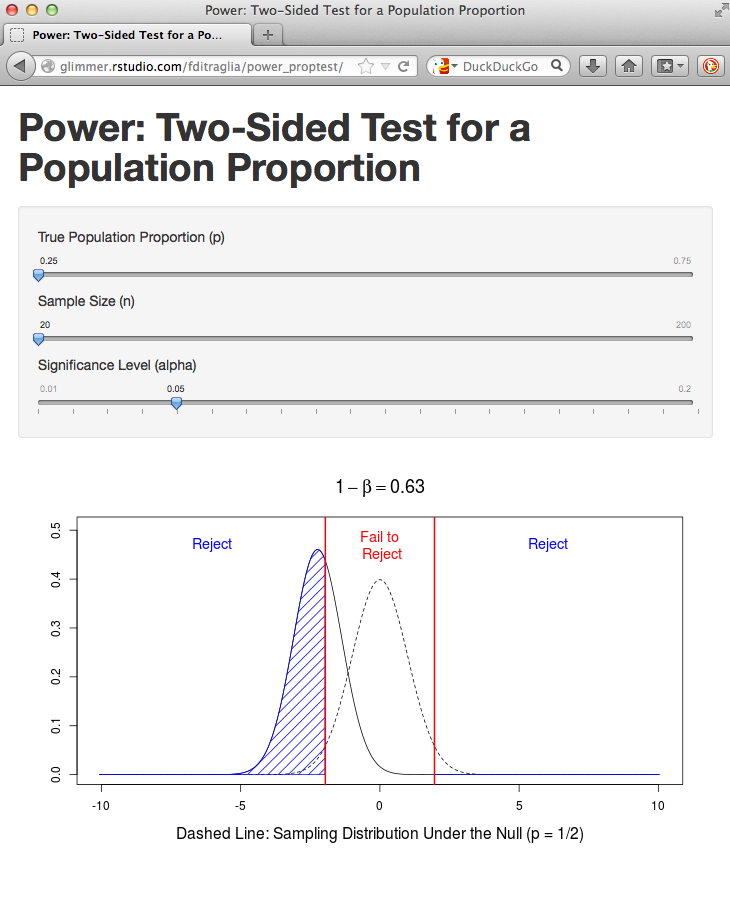
\includegraphics[scale = 0.22]{./images/power_proptest_screenshot}}
\end{figure}

\end{frame}
%%%%%%%%%%%%%%%%%%%%%%%%%%%%%%%%%%%%%%%%
\begin{frame}
\frametitle{Now We can Calculate Power!}
\small
\begin{block}{Decision Rule for Two-sided Test}
Reject $H_0\colon p = 0.5$ provided that $\alert{|T_n| \geq \texttt{qnorm}(1 - \alpha/2)}$
\end{block}

\begin{block}{If the null is false (i.e.\ under $H_1\colon p \neq 0.5$)}
	$$T_n = \frac{\widehat{p} - 0.5}{\sqrt{\frac{0.5(1-0.5)}{n}}} \approx N\left(\sqrt{n}(2p-1), 4 p(1-p)  \right)$$
\end{block}
\begin{block}{Thus, the probability of rejecting a false null is:}
	$$\boxed{\mbox{Power}(\alpha, p, n) = P\left( |Y| \geq c\right)  = P(Y \leq -c) + P(Y\geq c)}$$
		\begin{eqnarray*}
			 c &=&\texttt{qnorm}(1 - \alpha/2) \\
			 Y &\sim& N\left(\sqrt{n}(2p-1), 4 p(1-p)  \right)
		 \end{eqnarray*} 
\end{block}
\end{frame}
%%%%%%%%%%%%%%%%%%%%%%%%%%%%%%%%%%%%%%%%
\begin{frame}
	\frametitle{\href{http://glimmer.rstudio.com/fditraglia/power_proptest/}{http://glimmer.rstudio.com/fditraglia/power\_proptest/}}
\framesubtitle{Now look at everything and try changing all the sliders!}

\begin{figure}
	\fbox{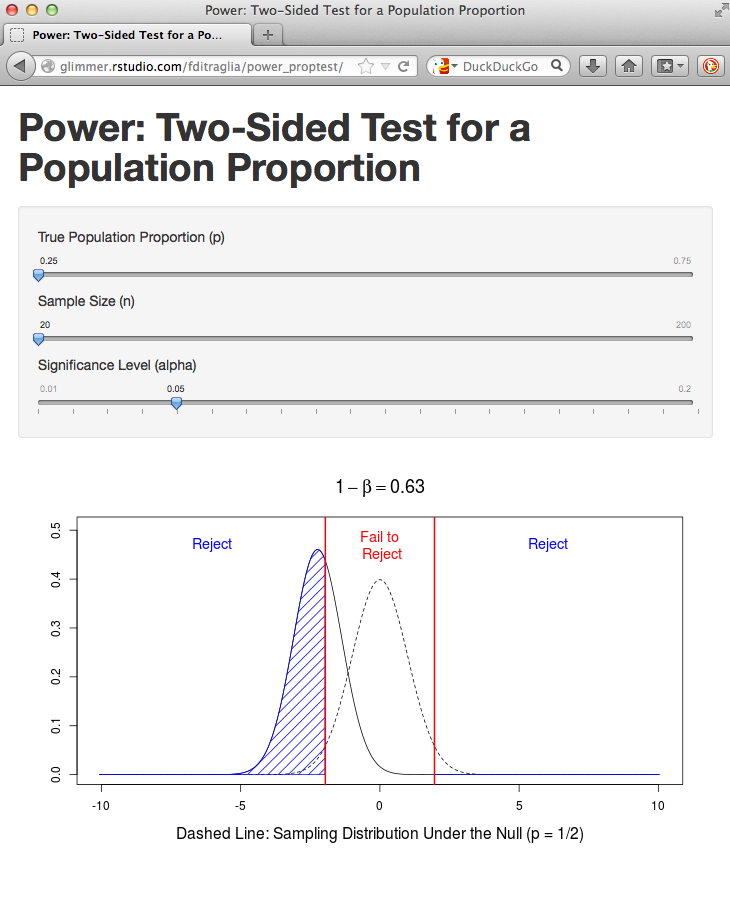
\includegraphics[scale = 0.22]{./images/power_proptest_screenshot}}
\end{figure}

\end{frame}
%%%%%%%%%%%%%%%%%%%%%%%%%%%%%%%%%%%%%%%%\begin{frame}
\begin{frame}
\begin{center}
	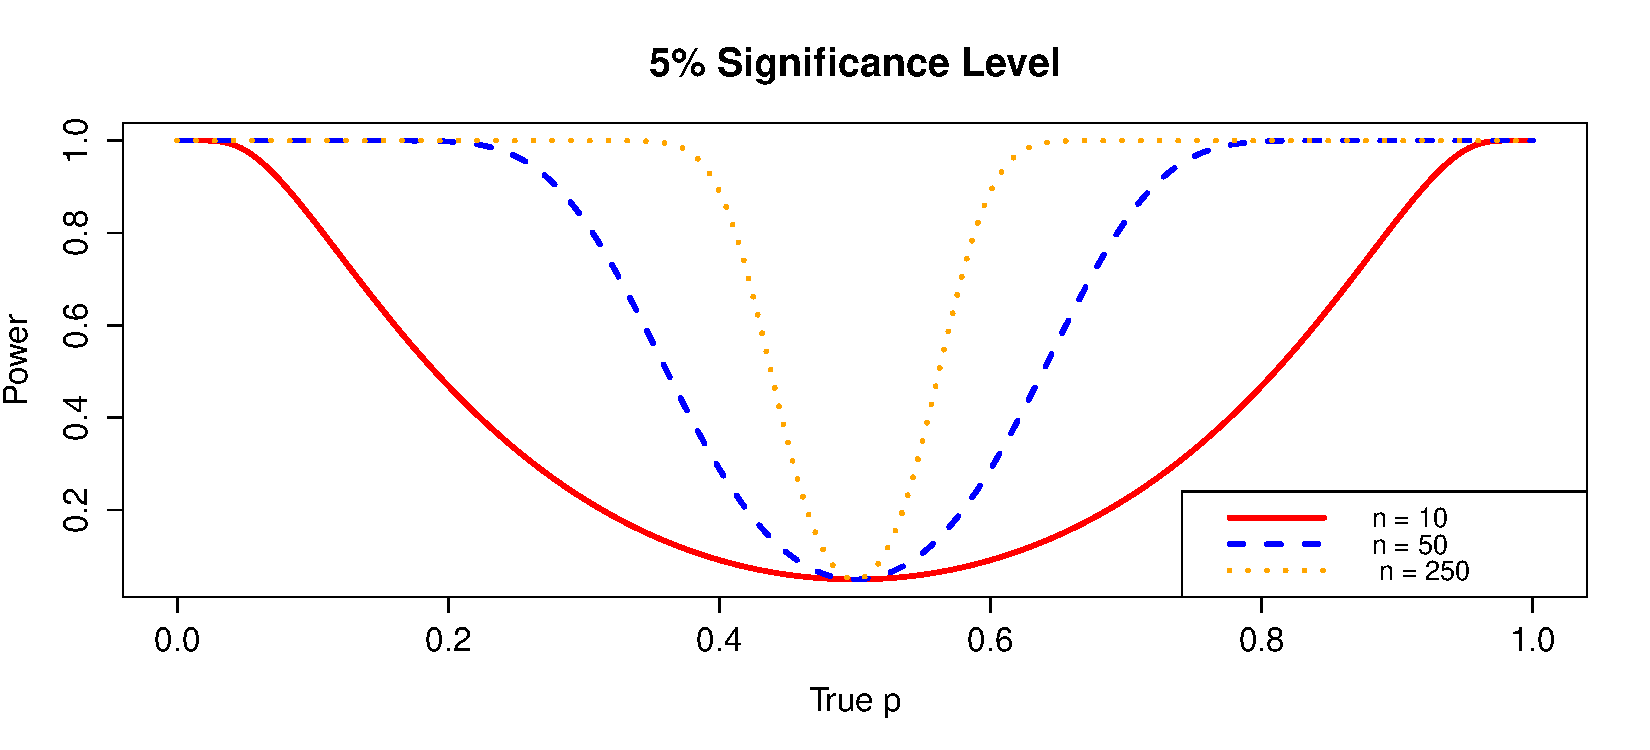
\includegraphics[scale=0.37]{./images/power_change_n}\\
	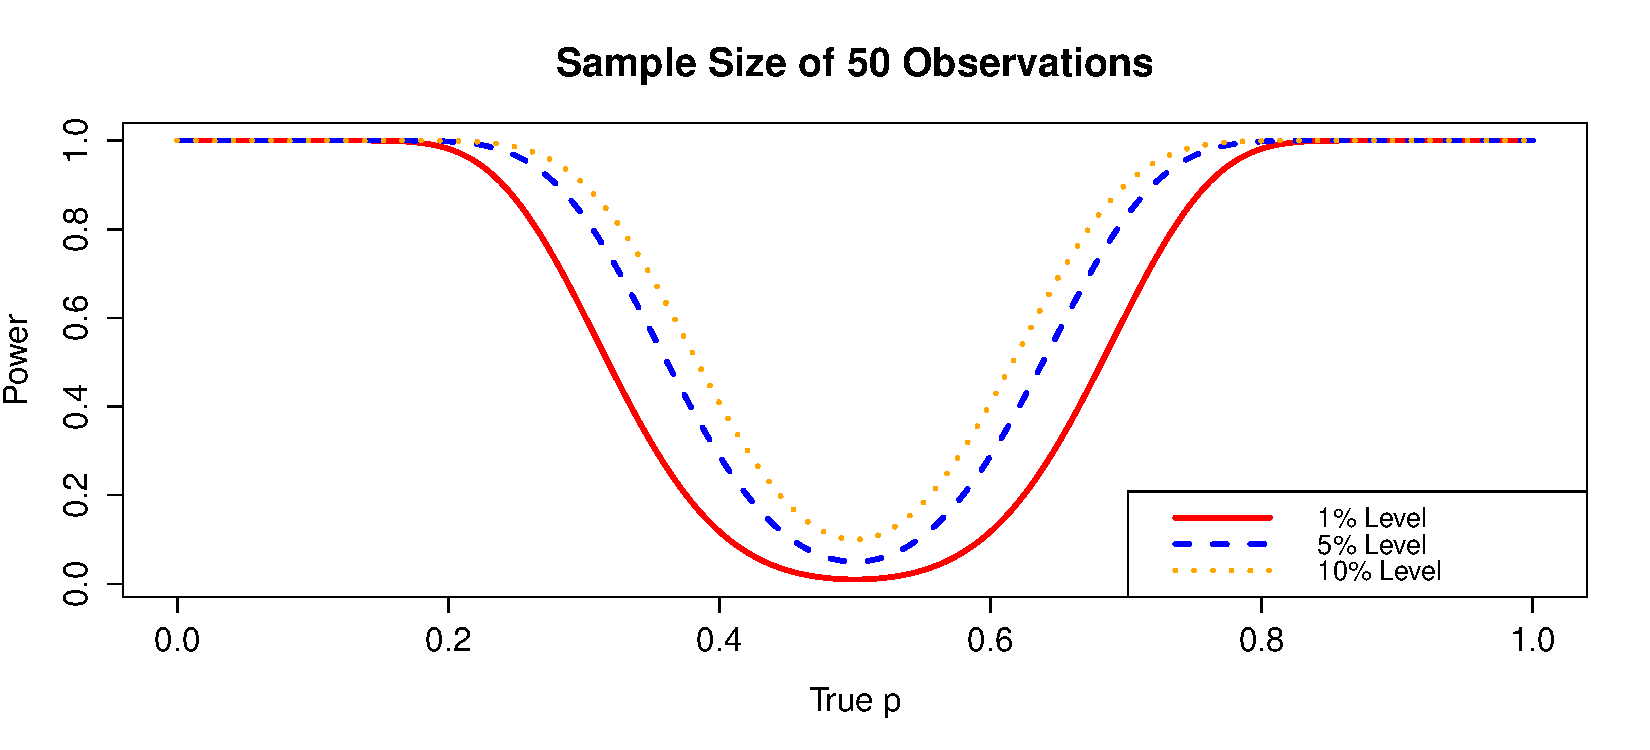
\includegraphics[scale=0.37]{./images/power_change_a}
\end{center}
\end{frame}
%%%%%%%%%%%%%%%%%%%%%%%%%%%%%%%%%%%%%%%%
\begin{frame}
\frametitle{Some Intuition about Power for the Coin Example}
\small
	\begin{itemize}
	\item Equals prob.\ of rejecting false null, i.e.\ convicting a guilty person.
	\item Tells us how large a sample we would need to detect a given discrepancy from ``fairness'' of the coin: $p = 0.5$
		\begin{itemize}
			\item Small deviations from $p=0.5$ unlikely to be detected unless the sample size is large.
			\item Large deviations from $p=0.5$ very likely to be detected even if the sample size is small.
		\end{itemize}
		\item For a \emph{given} degree of ``unfairness'' (deviation from $p = 0.5$)
			\begin{itemize}
				\item Higher significance level ($\alpha$) $\implies$ higher power ($1-\beta$)
				\item Large sample size ($n$) $\implies$ higher power ($1-\beta$)
			\end{itemize}
	\end{itemize}
\end{frame}

%%%%%%%%%%%%%%%%%%%%%%%%%%%%%%%%%%%%%%%%

\begin{frame}
\frametitle{Power More Generally}
	\begin{block}{Power $ = (1 - \beta) = 1 -  P$(Type II Error)}
Chance of detecting an effect given that one exists.
\end{block}
\begin{block}{Power Depends on Four Things}
	\begin{enumerate}
\item Magnitude of Effect: easier to detect large deviations from $H_0$
\item Amount of variability in the population: less variability $\implies$ easier to detect an effect of given size.
\item Sample Size: larger $n \implies$ easier to detect effect of given size
\item Signif.\ Level ($\alpha$): fewer Type I errors $\implies$ more Type II errors
\end{enumerate}
\end{block}
\alert{Go back and compare to factors that affect width of CI...}
\end{frame}
%%%%%%%%%%%%%%%%%%%%%%%%%%%%%%%%%%%%%%%%
% \begin{frame}
% \frametitle{An Important Point}
% For any discrepancy from $p = 0.5$, there is always a sample size large enough to make the power of our test \emph{arbitrarily close to one}. In other words, we can be almost certain to detect an effect, no matter how small, provided that we use a large enough sample. \alert{However, this does not mean that the affect we have found is important}.

% \vspace{2em}
% If it turned out that the true probability of heads was closer to 0.50001 rather than 0.5, should we really care? 
% \end{frame}
% %%%%%%%%%%%%%%%%%%%%%%%%%%%%%%%%%%%%%%%%
\begin{frame}[fragile]
\frametitle{An R Function to Calculate Power For Coin Example}
\footnotesize
	\begin{eqnarray*}
		\mbox{Power}(\alpha, p, n) &=& P\left(Y \leq -c\right) + P\left(Y\geq c\right)\\
			 c &=&\texttt{qnorm}(1 - \alpha/2) \\
			 Y &\sim& N\left(\sqrt{n}(2p-1), 4 p(1-p)  \right)
		 \end{eqnarray*} 

\begin{verbatim}
coin.power <- function(a, p, n){
    c <-  qnorm(1 - a/2)	
    mu <- sqrt(n) * (2 * p - 1) 	
    sigma <- sqrt(4 * p * (1 - p))
    
    less.than <- pnorm(-c, mean = mu, sd = sigma)
    greater.than <- 1 - pnorm(c, mean = mu, sd = sigma)
    power <- less.than + greater.than
    return(power)
}
\end{verbatim}
\end{frame}


%%%%%%%%%%%%%%%%%%%%%%%%%%%%%%%%%%%%%%%%

\begin{frame}[fragile]
\frametitle{Here's Some Code for You to Play Around With}
\footnotesize
You can use the function \texttt{coin.power} to calculate power for specific values of $p, n,$ and $\alpha$
\begin{verbatim}
coin.power(a = 0.05, p = 0.55, n = 100)
coin.power(a = 0.05, p = 0.55, n = 1000)
coin.power(a = 0.1, p = 0.55, n = 100)
coin.power(a = 0.05, p = 0.6, n = 100)
\end{verbatim}
or to make plots similar to those on slide 28
\begin{verbatim}
alternatives <- seq(from = 0, to = 1, by = 0.001)
power <- coin.power(a = 0.05, alternatives, n = 10)
plot(alternatives, power, xlab = `True p', ylab = `Power', type = `l')
\end{verbatim}
Try out different choices for $p,n$ and $\alpha$ and see what you get! I'll post this R code to save typing.

\end{frame}
%%%%%%%%%%%%%%%%%%%%%%%%%%%%%%%%%%%%%%%%

%%%%%%%%%%%%%%%%%%%%%%%%%%%%%%%%%%%%%%%%
% \begin{frame}
% \frametitle{Next Time}
% 	\begin{enumerate}
% 	\item Some final points about Hypothesis testing and CIs
% 	\item Regression Part II
% 	\end{enumerate}
% \end{frame}


%%%%%%%%%%%%%%%%%%%%%%%%%%%%%%%%%%%%%%%

\begin{frame}
\begin{center}
	\huge Some Final Thoughts on Hypothesis Testing and Confidence Intervals
\end{center}
\end{frame}
%%%%%%%%%%%%%%%%%%%%%%%%%%%%%%%%%%%%%%%%
\begin{frame}
\frametitle{Terminology I Have Intentionally Avoided Until Now}

\begin{block}{Statistical Significance}
Suppose we carry out a hypothesis test at the $\alpha\%$ level and,  based on our data, reject the null. You will often see this situation described as ``statistical significance.''
\end{block}

\begin{block}{In Other Words...}
When people say ``statistically significant'' what they really mean is that they rejected the null hypothesis.
\end{block}
\end{frame}

%%%%%%%%%%%%%%%%%%%%%%%%%%%%%%%%%%%%%%%
\begin{frame}
\frametitle{Some Examples}

	\begin{itemize}
		\item We found a difference between the ``Hi'' and ``Lo'' groups in the anchoring experiment that was statistically significant at the 5\% level based on data from a past semester.
		\item Our 95\% CI for the proportion of US voters who know who John Roberts is did not include 0.5. Viewed as a two-sided test, we found that the difference between the true population proportion and 0.5 was statistically significant at the 5\% level.
	\end{itemize}

\end{frame}
%%%%%%%%%%%%%%%%%%%%%%%%%%%%%%%%%%%%%%%
\begin{frame}
\frametitle{Why Did I Avoid this Terminology?}
\small
\begin{block}{Statistical Significance $\neq$ Practical Importance}
	\begin{itemize}
		\item You need to understand the term ``statistically significant'' since it is widely used. A better term for the idea, however, would be ``statistically discernible''
		\item Unfortunately, many people are confuse ``significance'' in the narrow, technical sense with the everyday English word meaning ``important'' 
		\item \alert{Statistically Significant Does Not Mean Important!"}
			\begin{itemize}
				\item A difference can be practically unimportant but statistically significant.
				\item A difference can be practically important but statistically insignificant.
			\end{itemize}
	\end{itemize}
\end{block}


\end{frame}


%%%%%%%%%%%%%%%%%%%%%%%%%%%%%%%%%%%%%%%
\begin{frame}
\begin{center}
\Huge P-value Measures Strength of Evidence Against $H_0$\\ \alert{Not The Size of an Effect!}
\end{center}
\end{frame}
%%%%%%%%%%%%%%%%%%%%%%%%%%%%%%%%%%%%%%%
\begin{frame}
\frametitle{Statistically Significant but Not Practically Important}
\small
I flipped a coin 10 million times (in R) and got 4990615 heads.
\begin{block}{Test of $H_0\colon p = 0.5$ against $H_1\colon p \neq 0.5$}
$$T = \displaystyle \frac{\widehat{p} - 0.5}{\sqrt{0.5(1-0.5)/n}} \approx -5.9   \implies \alert{\mbox{ p-value } \approx 0.000000003}$$
\end{block}

\begin{block}{Approximate 95\% Confidence Interval}
 $$\widehat{p} \pm \texttt{qnorm}(1 - 0.05/2) \sqrt{\frac{\widehat{p}(1-\widehat{p})}{n}}  \implies \alert{(0.4988, 0.4994)}$$
\end{block}

\footnotesize (Such a huge sample size that refined vs.\ textbook CI makes no difference)
\large
\vspace{1em}

\alert{\fbox{Actual $p$ was 0.499}}
\end{frame}

%%%%%%%%%%%%%%%%%%%%%%%%%%%%%%%%%%%%%%%

\begin{frame}
\frametitle{Practically Important But Not Statistically Significant}
\framesubtitle{\href{http://www.amazon.com/p-value-Stories-Actually-Understand-Statistics/dp/0321629302}{\fbox{Vickers: ``What is a P-value Anyway?'' (p. 62)}}}
\footnotesize
\begin{quote}
Just before I started writing this book, a study was published reporting about a 10\% lower rate of breast cancer in women who were advised to eat less fat. If this indeed the true difference, low fat diets could reduce the incidence of breast cancer by tens of thousands of women each year -- astonishing health benefit for something as simple and inexpensive as cutting down on fatty foods. The p-value for the difference in cancer rates was 0.07 and here is the key point: this was widely misinterpreted as indicating that low fat diets don't work. For example, the \emph{New York Times} editorial page trumpeted that ``low fat diets flub a test'' and claimed that the study provided ``strong evidence that the war against all fats was mostly in vain.'' \alert{However failure to prove that a treatment is effective is not the same as proving it ineffective.}
\end{quote}
\end{frame}
%%%%%%%%%%%%%%%%%%%%%%%%%%%%%%%%%%%%%%%
\begin{frame}[c]\frametitle{Do Students with 4-Letter Surnames Do Better?}
 \framesubtitle{Based on Data from Midterm 1}
    \begin{columns}
    	\column{0.35\textwidth} \begin{block}
    		{4-Letter Surname}
    			$\bar{x} = 88.9$\\
    			$s_x = 10.4$\\
    			$n_x = 12$
    	\end{block} 
    	\column{0.35\textwidth} \begin{block}
    		{Other Surnames}
    			$\bar{y} = 74.4$\\
    			$s_y = 20.7$\\
    			$n_y = 92$
    	\end{block}
    \end{columns}

\vspace{1em}
\begin{block}
	{Difference of Means}
	$\bar{x} - \bar{y} = \alert{14.5}$
\end{block}
\begin{block}
	{Standard Error}
	$\displaystyle SE = \sqrt{s_x^2/n_x + s_y^2/n_y} \approx \alert{3.7}$
\end{block}
\begin{block}
	{Test Statistic}
	$T = 14.5 / 3.7 \approx \alert{3.9}$
\end{block}
\end{frame}
%%%%%%%%%%%%%%%%%%%%%%%%%%%%%%%%%%%%%%%
\begin{frame}[c]\frametitle{What is the p-value for the two-sided test?  \hfill 
\includegraphics[scale = 0.05]{./images/clicker}}
    
$$\boxed{\mbox{Test Statistic} \approx 3.9}$$

\begin{enumerate}[(a)]
	\item $p < 0.01$
	\item $0.01 \leq p < 0.05$
	\item $0.05 \leq p < 0.1$
	\item $p > 0.1$
	\item Not Sure
\end{enumerate}
\end{frame}
%%%%%%%%%%%%%%%%%%%%%%%%%%%%%%%%%%%%%%%
\begin{frame}[c]\frametitle{What do these results mean? \hfill 
\includegraphics[scale = 0.05]{./images/clicker}}

Evaulate this statement in light of our hypothesis test:
\vspace{1em}

\begin{quote}
	Students with four-letter long surnames do better, on average, on the first midterm of Econ 103 at UPenn.
\end{quote}

\begin{enumerate}[(a)]
	\item Strong evidence in favor
	\item Moderate evidence in favor
	\item No evidence either way
	\item Moderate evidence against
	\item Strong evidence against
\end{enumerate}
\end{frame}
%%%%%%%%%%%%%%%%%%%%%%%%%%%%%%%%%%%%%%%
\begin{frame}[c,fragile]\frametitle{I just did 134 Hypothesis Tests...}
   
 \begin{block}
 	{... and 11 of them were significant at the 5\% level.}
 \end{block}

\footnotesize

\begin{verbatim}
         group sign p.value x.bar N.x  s.x y.bar N.y  s.y
26  first1 = P    1   0.000  93.8   3  2.9  75.5 101 20.4
70     id2 = 7    1   0.000  94.6   5  3.3  75.1  99 20.4
134    id8 = 0    1   0.000  92.6   7  4.9  74.8  97 20.5
5    Nlast = 4    1   0.001  88.9  12 10.4  74.4  92 20.7
90     id4 = 8    1   0.003  87.7   9  9.0  74.9  95 20.7
105    id6 = 8    1   0.003  88.1   5  5.8  75.4  99 20.6
109    id6 = 2    1   0.007  88.9   8 10.7  75.0  96 20.6
9    Nlast = 2    1   0.016  90.4   5  9.3  75.3  99 20.5
49   last1 = P   -1   0.036  65.2   6  9.9  76.7  98 20.6
65     id2 = 1    1   0.038  84.3   9 10.1  75.3  95 20.9
117    id7 = 8    1   0.041  83.4  13 11.6  75.0  91 21.1
\end{verbatim}
\end{frame}


%%%%%%%%%%%%%%%%%%%%%%%%%%%%%%%%%%%%%%%
% \begin{frame}
% \frametitle{Green Jelly Beans Cause Acne!}
% \framesubtitle{\href{http://xkcd.com/882/}{\fbox{xkcd \#882}}}
% \begin{center}
% 	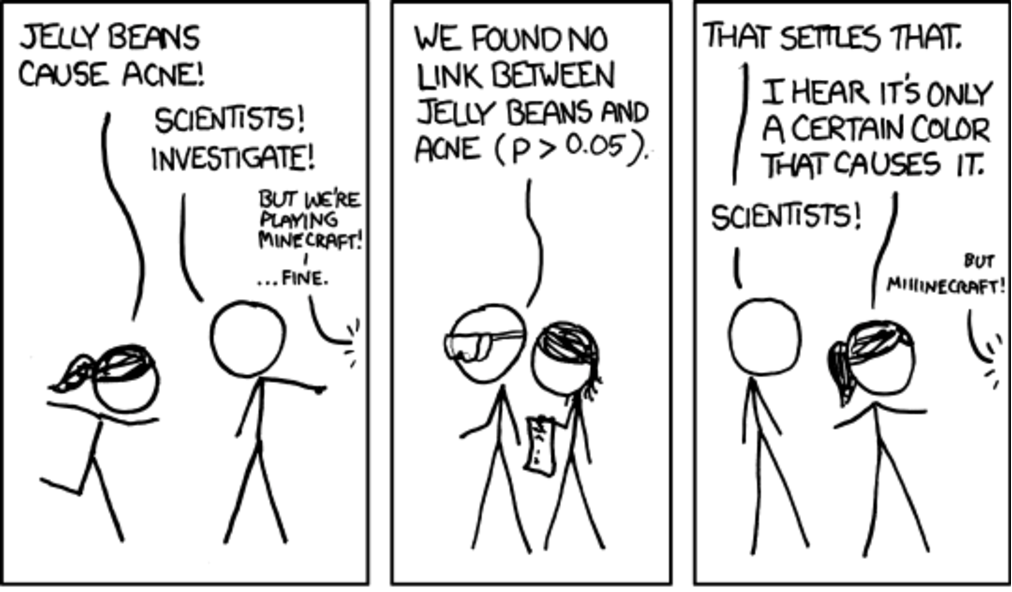
\includegraphics[scale=0.45]{./images/xkcd1}
% \end{center}
% \end{frame}
% %%%%%%%%%%%%%%%%%%%%%%%%%%%%%%%%%%%%%%%%
% \begin{frame}
% \begin{center}
% 	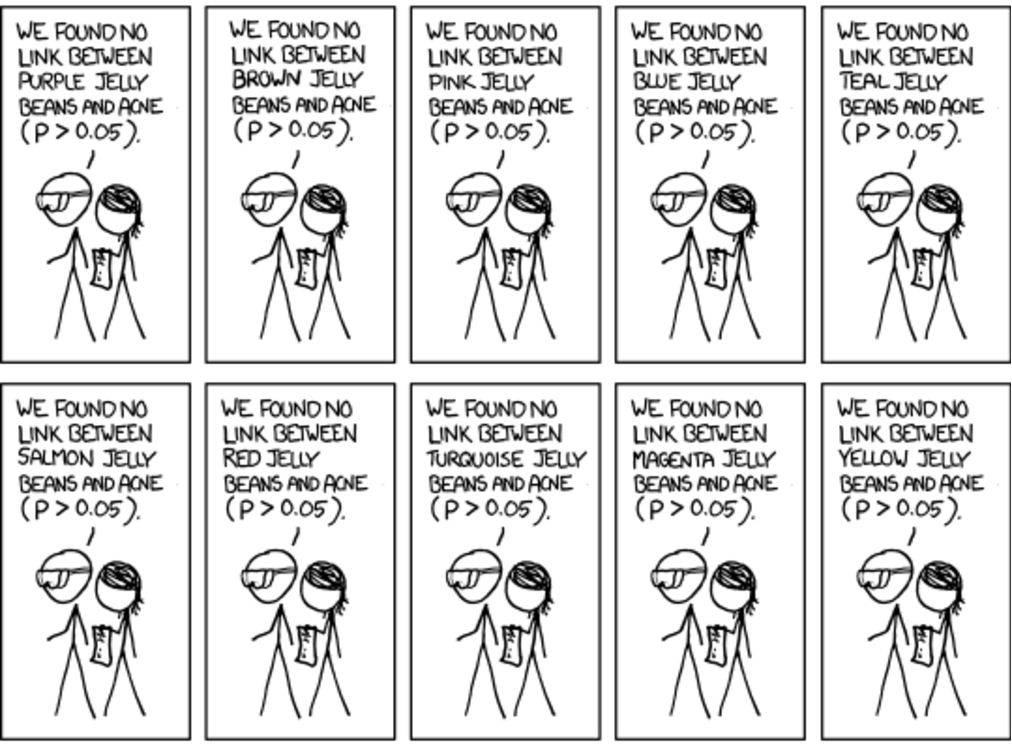
\includegraphics[scale=0.45]{./images/xkcd2}

% \end{center}
% \end{frame}
% %%%%%%%%%%%%%%%%%%%%%%%%%%%%%%%%%%%%%%%%
% \begin{frame}
% \begin{center}
% 	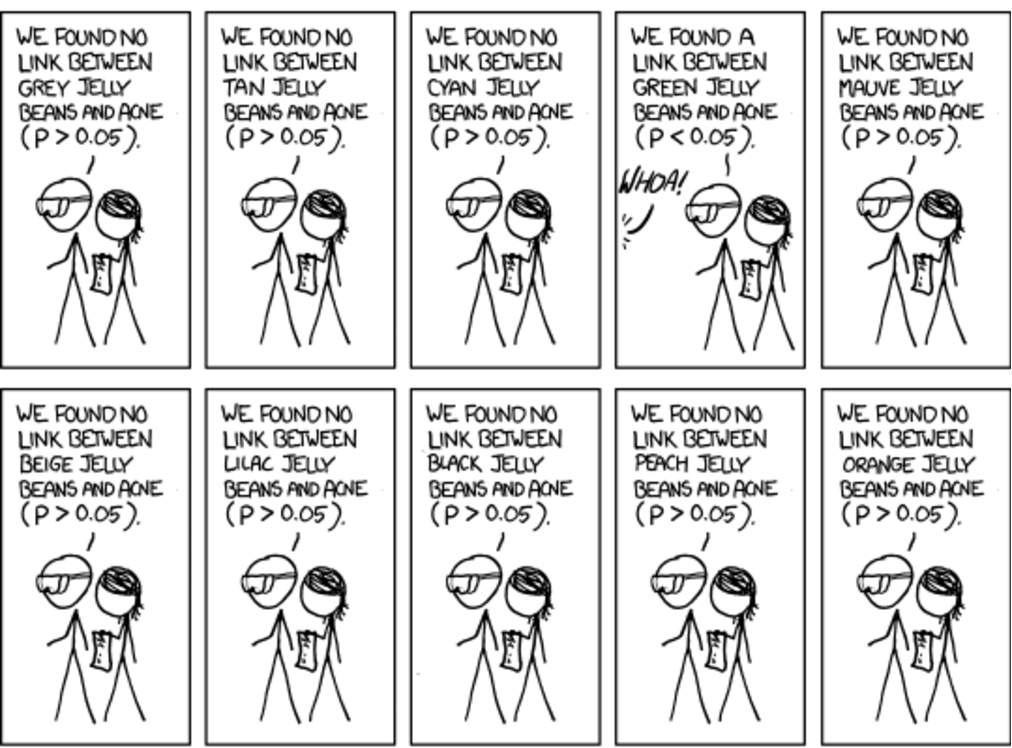
\includegraphics[scale=0.45]{./images/xkcd3}

% \end{center}
% \end{frame}
% %%%%%%%%%%%%%%%%%%%%%%%%%%%%%%%%%%%%%%%%
% \begin{frame}
% \begin{center}
% 	
\includegraphics[scale=0.45]{./images/xkcd4}

% \end{center}
% \end{frame}
% %%%%%%%%%%%%%%%%%%%%%%%%%%%%%%%%%%%%%%%%
% \begin{frame}
% \frametitle{\hfill 
\includegraphics[scale = 0.05]{./images/clicker}}
% Ignoring outside information, that is strictly on the basis of the hypothesis tests presented in the cartoon, do you think we have reason to believe that green jelly beans are linked to acne?
% 	\begin{enumerate}[(a)]
% 		\item Yes
% 		\item No
% 		\item Not Sure
% 	\end{enumerate}

% \end{frame}
%%%%%%%%%%%%%%%%%%%%%%%%%%%%%%%%%%%%%%%%
\begin{frame}
\frametitle{Data-Dredging}
\begin{itemize}
	\item Suppose you have a long list of null hypotheses and assume, for the sake of argument that all of them are true.
		\begin{itemize}
			\item E.g.\ there's no difference in grades between students with different 4th digits of their student id number. 
		\end{itemize}
	\item We'll still reject about 5\% of the null hypotheses.
	\item Academic journals tend only to publish results in which a null hypothesis is rejected at the 5\% level or lower. 
	\item We end up with the bizarre result that ``most published studies are false.''  
\end{itemize}


\alert{I posted a reading about this on Piazza: ``The Economist - Trouble in the Lab.'' To learn even more, see \href{http://www.plosmedicine.org/article/info:doi/10.1371/journal.pmed.0020124}{\textcolor{blue}{\fbox{Ioannidis (2005)}}}}


\end{frame}
%%%%%%%%%%%%%%%%%%%%%%%%%%%%%%%%%%%%%%%%
\begin{frame}
\frametitle{Green Jelly Beans Cause Acne!}
\framesubtitle{\href{http://xkcd.com/882/}{\fbox{xkcd \#882}}}
\begin{figure}
\centering
	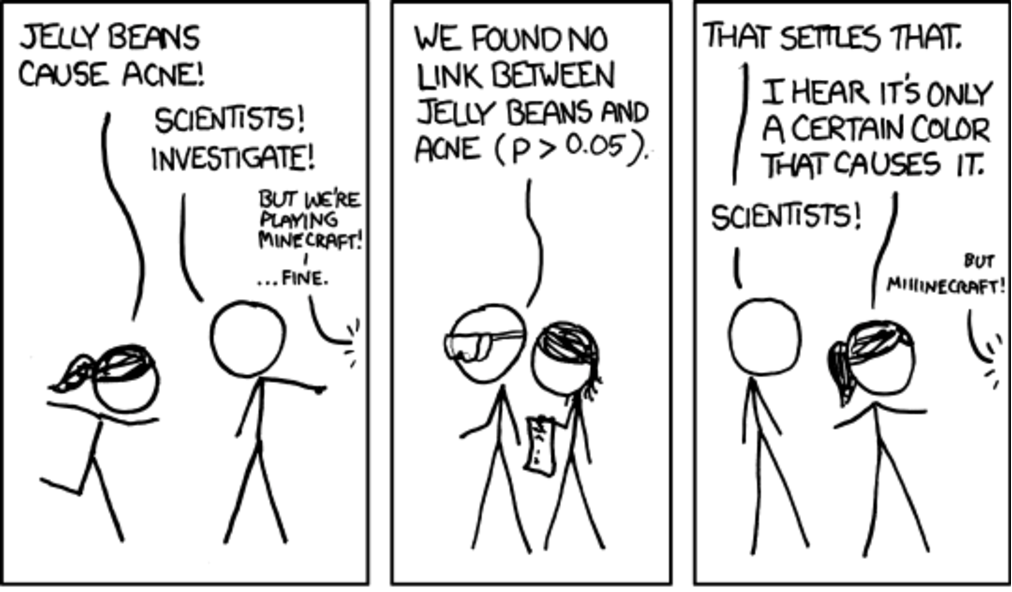
\includegraphics[scale=0.45]{./images/xkcd1}
	\caption{Go and read this comic strip: before today's lecture you wouldn't have gotten the joke!}
\end{figure}
\end{frame}
%%%%%%%%%%%%%%%%%%%%%%%%%%%%%%%%%%%%%%%%

% \begin{frame}
% \frametitle{Don't Compare P-Values Across Different Tests!}
% \framesubtitle{\fbox{\href{http://www.people-press.org/files/2012/08/8-10-12-Knowledge-release.pdf}{Pew: ``What Voters Know About Campaign 2012''}}}


% \footnotesize

% Of 239 Republicans, 61\% knew Romney is pro-life vs.\ 53\% of 238 Democrats.
% \pause
% \begin{block}{$H_0\colon p_{Rep} = 0.5$ vs.\ $H_1\colon p_{Rep} \neq 0.5$}
%  $$T = \frac{0.61 - 0.5}{\sqrt{0.5(1-0.5)/239}} \approx  3.4 \implies \mbox{ p-value } \approx 0.0007$$
% \end{block}
% \pause
% \begin{block}{$H_0\colon q_{Dem} = 0.5$ vs.\ $H_1\colon q_{Dem} \neq 0.5$}
%  $$T = \frac{0.53 - 0.5}{\sqrt{0.5(1-0.5)/238}} \approx 0.93  \implies \mbox{ p-value } \approx 0.35$$
% \end{block}
% \pause
% \begin{block}{$H_0\colon p_{Rep} =q_{Dem}$ vs.\ $H_1\colon p_{Rep} \neq q_{Dem}$}
%  $$T = \frac{0.61 - 0.53}{\sqrt{\left(\frac{1}{239}+ \frac{1}{238}\right)\left(\frac{239 \times 0.61 + 238 \times 0.53}{239 + 238}\right)}} \approx  1.76 \implies \mbox{ p-value } \approx 0.08$$
% \end{block}


% \end{frame}

%%%%%%%%%%%%%%%%%%%%%%%%%%%%%%%%%%%%%%%%
% \begin{frame}
% \frametitle{Don't Compare P-Values Across Different Tests!}

% \begin{itemize}
% 	\item P-Value measures strength of evidence against the null, not the size of an affect! \pause
% 	\item Use a single test to address a single research question: if you are actually interested in differences between Republicans and Democrats, test for this directly! \pause
% \end{itemize}

% \vspace{1em}

% \pause

% For more on the problems associated with comparing p-values from different hypothesis tests, along with an even starker example than the one I just showed you, see \href{http://amstat.tandfonline.com/doi/abs/10.1198/000313006X152649}{\textcolor{blue}{\fbox{Gelman \& Stern (2006)}}}

% \end{frame}


%%%%%%%%%%%%%%%%%%%%%%%%%%%%%%%%%%%%%%%%

\begin{frame}
\frametitle{Some Final Thoughts}
	\begin{itemize}
		\item Failing to reject $H_0$ does not mean $H_0$ is true. 
		\item Rejecting $H_0$ does not mean $H_1$ is true.
		\item P-values are always more informative than simply reporting ``Reject'' vs.\ ``Fail To Reject'' at a given significance level. 
		\item Confidence intervals are more informative that hypothesis tests, since they give an idea of the size of an effect. 
		\item If $H_0$ is actually plausible a priori (this is rarer than you may think), reporting a p-value can be a good complement to a CI. 
		\item To avoid data-dredging be honest about the tests you have carried out: report \emph{all of them}, not just the ones where you rejected the null.
	\end{itemize}

\end{frame}
\end{document}